\renewcommand{\nomducours}{\nomcoursdeux}
\renewcommand{\chapterlabel}{chap_deux}
\renewcommand{\sousnomducours}{\sousnomcoursdeux}
\renewcommand{\contentsummaryducours}{\contentsummarycoursdeux}

\chapter{\nomducours}
\thispagestyle{empty}
\label{\chapterlabel}

\begin{tetedechapitre}[\contentsummaryducours]
	Nous commençons notre étude de la thermodynamique en nous concentrant sur une quantité de masse fixe. Ce \coursdeux se propose de répondre à deux questions :
\begin{itemize}
	\item Comment quantifier le travail que peut recevoir et fournir un corps de masse~fixe ?
	\item Qu’est-ce que la réversibilité, pourquoi et comment l’atteindre ?
\end{itemize}
\par
\end{tetedechapitre}

\section{Pourquoi utiliser un système fermé ?}

		À partir de maintenant, nous voulons décrire et quantifier les transferts d’énergie dans les fluides. Nous pouvons adopter deux points de vue différents pour observer le fluide :
		\begin{itemize}
			\item Soit nous «~découpons~» un petit morceau de masse, que nous suivons de près lorsqu’il évolue, puis nous quantifions l’énergie qui lui est transférée : c’est ce que nous appelons un \vocab{système fermé} ;
			\item Soit nous choisissons un morceau de volume fixe, qui est \emph{traversé} en permanence par un débit de masse, puis nous quantifions les transferts d’énergie vers le volume : c’est ce que nous appelons un \vocab{système ouvert}.
		\end{itemize}
		
		Bien sûr, ces deux méthodes sont équivalentes : elles vont produire les mêmes résultats. Le choix de l’une ou l’autre rendra simplement l’analyse et la quantification des transferts plus aisée.

		\begin{figure}
			\begin{center}
			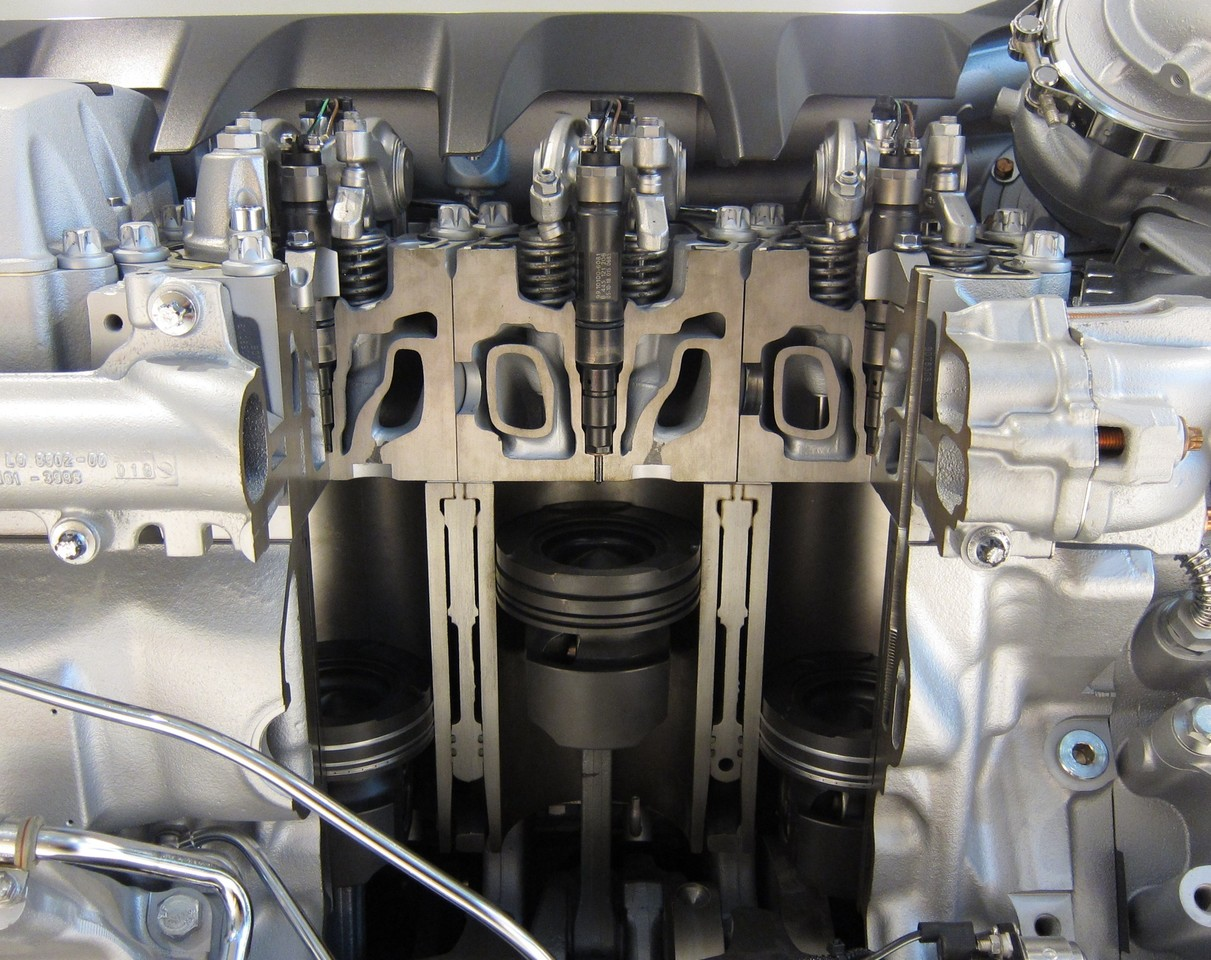
\includegraphics[width=8cm]{images/diesel_engine_cutaway.jpg}
			\end{center}
			\supercaption{Une découpe dans un moteur de camion laisse apparaître trois pistons dans leurs cylindres. Un système fermé est un bon outil pour étudier l’air emprisonné dans un cylindre. Le moteur photographié est un diesel \textsc{man} en V8.}%
				{\wcfile{Cutaway of a MAN V8 Diesel engine.jpg}{Photo} \ccbysa \olivier}
				\label{fig_diesel_engine_cutaway}
		\end{figure}
		
		L’utilisation d’un système fermé est judicieuse pour analyser les machines à mouvement alternatif (moteurs automobiles, pompes et compresseurs et généralement toutes les machines à pistons/cylindres). Ces machines divisent le fluide en petites quantités qui sont emprisonnées dans une enclave, dans laquelle elles sont chauffées, refroidies, comprimées ou détendues (\cref{fig_diesel_engine_cutaway}). Il est alors facile d’identifier une quantité de masse donnée et de quantifier les transferts qu’elle subit.
		
		À l’inverse, pour étudier ce qui se passe dans une tuyère de turboréacteur par exemple, nous aurions des difficultés pour identifier un groupe donné de particules et quantifier le changement de ses propriétés. Il sera alors judicieux d’utiliser un système ouvert, comme nous l’étudierons au \courstrois.
		
		Concrètement, dans ce chapitre, nous voulons quantifier le travail qu’on peut générer avec un fluide dans un cylindre. Un moteur de voiture fournit du travail parce que l’air dans les cylindres fournit plus de travail en se détendant au retour qu’il n’en a reçu à en se faisant comprimer à l’aller (\cref{fig_moteur_sf}). Comment peut-on générer cela ? Pour répondre à cette question, il nous faut une méthode robuste pour quantifier les transferts d’énergie.

		\begin{figure}
			\begin{center}
			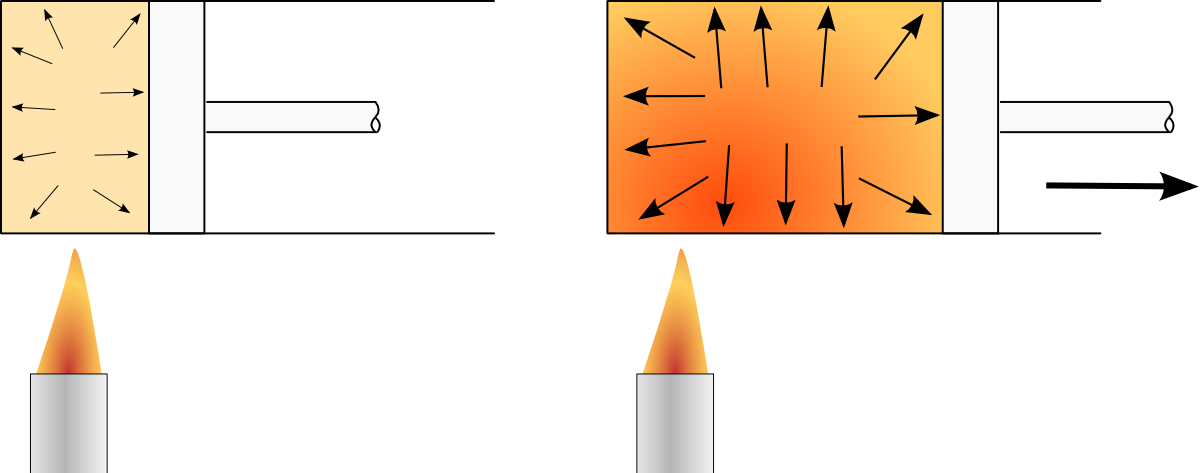
\includegraphics[width=\textwidth]{images/fonctionnement_base_moteur.png}
			\end{center}
			\supercaption{Principe de fonctionnement d’un moteur. Lorsque l’on fournit de la chaleur à un fluide dans un réservoir fermé, celui-ci augmente les forces qu’il exerce sur les parois du réservoir. En laissant le réservoir se déformer, on fait effectuer un travail au fluide.}{schéma \cczero \oc}
			\label{fig_moteur_sf}
		\end{figure}


\section{Conventions de comptabilité}
\label{ch_conventions_compta_sf}

	\subsection{Le système fermé}

			Nous appelons \vocab{système fermé} un sujet d’étude arbitraire dont les frontières sont imperméables à la masse : un ensemble donné de particules, de masse fixe. Toutes les propriétés de cet ensemble (pression, température, volume, etc.) peuvent être amenées à changer, mais il s’agit toujours des mêmes molécules, non mélangées à d’autres. Par exemple, un gaz prisonnier dans un cylindre et comprimé par un piston (\cref{fig_piston_m_cste}) est parfaitement décrit avec un système fermé.

		\begin{figure}
			\begin{center}
			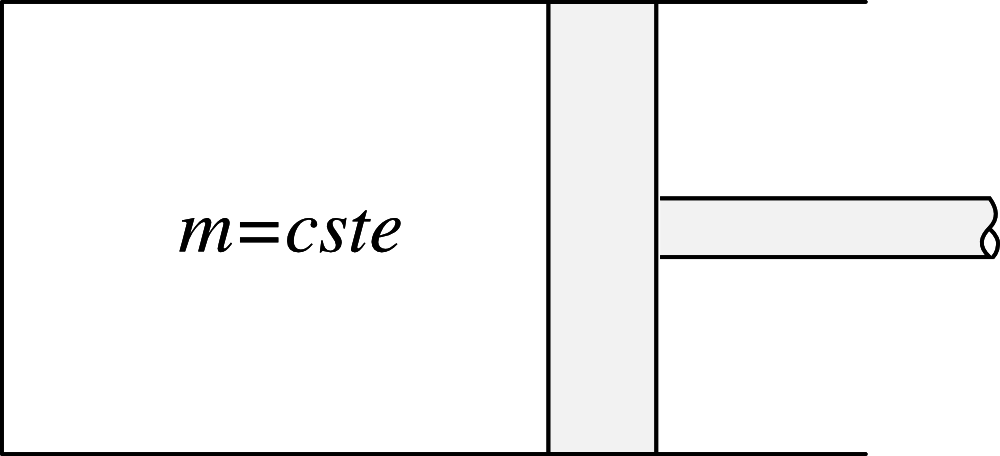
\includegraphics[width=6cm]{images/piston_cylindre.png}
			\end{center}
			\supercaption{Un système fermé typique : une quantité de masse fixe dans un réservoir fermé.
Une paroi mobile permet de la comprimer ; nous lui ferons également recevoir et perdre de la chaleur.}{schéma \cczero \oc}
			\label{fig_piston_m_cste}
		\end{figure}

	\subsection{Conventions de signe}
	\label{ch_convention_signe_sf}

		Pour quantifier les transferts nous utiliserons la convention de signe suivante, illustrée en \cref{fig_convention_signe_sf} :

		\begin{itemize}
			\item Lorsqu’ils sont positifs, les transferts $Q$ et $W$ traduisent une \emph{réception} par le système.
			\item À l’inverse, lorsqu’ils sont négatifs, les transferts $Q$ et $W$ indiquent une \emph{perte} du système. Le travail $W$ est alors fourni et la chaleur $Q$ émise.
		\end{itemize}

		\begin{figure}
			\begin{center}
				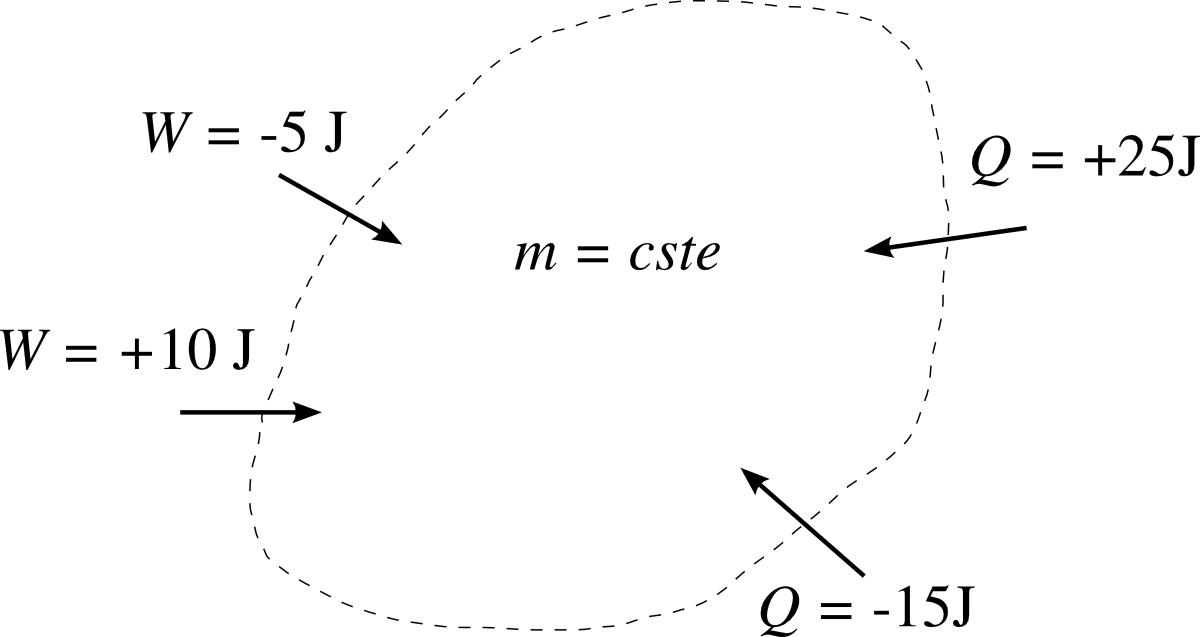
\includegraphics[width=9cm]{images/convention_systeme_ferme.png}
			\end{center}
			\supercaption{Conventions de signe pour un système fermé. Les flux entrants sont positifs, les flux sortants sont négatifs ; ils sont tous représentés avec des flèches rentrantes. La quantité de masse est fixe.}{schéma \cczero \oc}
			\label{fig_convention_signe_sf}
		\end{figure}

		Ainsi, dans les équations, nous pouvons systématiquement additionner les termes sans avoir à connaître le sens des transformations. Les transferts sont comptabilisés comme sur un compte bancaire : les dépenses sont négatives et les recettes positives.



\section{Le premier principe dans un système fermé}
\label{ch_premier_principe_sf}

	\thermoquotebegin{O}
		Appelons ainsi $Q$ la quantité totale de chaleur qui doit être impartie à un corps pendant son passage, d’une manière donnée, depuis une condition à une autre, (toute chaleur prélevée au corps étant comptée comme une quantité négative), alors nous la divisons en trois parties, parmi lesquelles la première est employée à augmenter la chaleur existant véritablement dans le corps, la seconde à produire le travail intérieur et la troisième à produire le travail extérieur. Il va de la seconde partie ce que nous avons déjà dit de la première : qu’elle est indépendante du chemin suivi dans le passage du corps d’un état à un autre, et nous pouvons en conséquence représenter ces deux parties ensemble par une fonction $U$, qui même si nous ne pouvons mieux la définir, nous savons à l’avance au moins être entièrement déterminée par les états initial et final du corps.
	\thermoquoteend{Rudolf Clausius, 1854}{\textit{Über eine veränderte Form des zweiten Hauptsatzes der mechanischen Wärmetheorie~\cite{clausius1854}}\vspace{1em}} %handmade vspace
	Le premier principe stipule que l’énergie est indestructible (\S\ref{ch_premier_principe}). Si on fournit \SI{100}{\joule} de travail à un système fermé et qu’il perd \SI{80}{\joule} sous forme de chaleur, c’est donc que «~son~» énergie a augmenté de~\SI{20}{\joule}. Nous nommons cette variation la \vocab{variation d’énergie interne}, $\Delta U$.
	
	Sous forme d’équation, le premier principe dans un système fermé se traduit par l’équation :
	\begin{equation}
		Q_{1 \to 2} + W_{1 \to 2} = \Delta U
		\label{eq_premier_principe_sf_maj}
	\end{equation}
	\begin{equationterms}
		\item pour un système fermé immobile ;
		\item où \tab $\Delta U = U_2 - U_1$ est la variation d’énergie interne (\si{\joule}),
		\item 	\tab $W_{1 \to 2}$ 	\tab est le travail reçu par le système (\si{\joule}),
		\item et \tab $Q_{1 \to 2}$ 	\tab est la chaleur reçue par le système (\si{\joule}).
	\end{equationterms}

	Malheureusement l’énergie interne $U$ est parfois très difficile à mesurer. Nous verrons dans les chapitres~\quatre et~\cinq que les corps emmagasinent cette énergie interne de différentes façons, et qu’elle est intimement liée à la température. L’énergie interne $U$, par définition, est toujours positive, mais sa variation $\Delta U$ ne l’est pas nécessairement.

	L’\cref{eq_premier_principe_sf_maj} peut être exprimée avec des grandeurs spécifiques :
	\begin{IEEEeqnarray}{rCl}
		m \ ( q_{1 \to 2} + w_{1 \to 2} )		& = & m \ \Delta u \nonumber \\
		q_{1 \to 2} + w_{1 \to 2} 				& = & \Delta u
	\label{eq_premier_principe_sf_min}
	\end{IEEEeqnarray}
	\begin{equationterms}
		\item pour un système fermé immobile ;
		\item où \tab $\Delta u = u_2 - u_1$ est la variation d’énergie interne spécifique (\si{\joule\per\kilogram}),
		\item 	\tab $w_{1 \to 2}$ 	\tab est le travail spécifique reçu par le système (\si{\joule\per\kilogram}),
		\item et \tab $q_{1 \to 2}$ 	\tab\tab est la chaleur spécifique reçue par le système (\si{\joule\per\kilogram}).
	\end{equationterms}
	
	Nous pouvons encore ré-écrire cette \cref{eq_premier_principe_sf_min} pour l’exprimer sous sa \vocab{forme différentielle} :
	\begin{IEEEeqnarray}{rCl}
		\diff q + \diff w	& = & \delta u
	\label{eq_premier_principe_sf_diff}
	\end{IEEEeqnarray}
	\begin{equationterms}
		\item pour un système fermé immobile ;
		\item où \tab $\delta u$ 	\tab\tab est la variation infinitésimale d’énergie interne spécifique (\si{\joule\per\kilogram}),
		\item 	\tab $\diff w$ 	\tab est le transfert infinitésimal de travail spécifique (\si{\joule\per\kilogram}),
		\item et \tab $\diff q$ 	\tab est le transfert infinitésimal de chaleur spécifique (\si{\joule\per\kilogram}).
	\end{equationterms}

	Dans cette \cref{eq_premier_principe_sf_diff}, les opérateurs $\diff$ et $\delta$ ont le même sens mathématique (celui de quantités infinitésimales) mais des significations phyiques différentes : $\diff w$ représente un \emph{transfert} infinitésimal qui s’intégrera en $w_{1 \to 2}$, tandis que $\delta u$ représente une \emph{variation} infinitésimale qui s’intégrera en $\Delta u = u_2 - u_1$.
	
	Lorsqu’un fluide est ramené à son état initial (même pression, même volume, même température), alors il contient exactement la même quantité d’énergie interne qu’auparavant. La totalité de l’énergie qu’il a reçue (sous forme de chaleur ou de travail) a donc nécessairement été rendue à l’extérieur sous une forme ou une autre. Nous exprimons cette affirmation ainsi :
	\begin{equation}
	Q_{\text{cycle}} + W_{\text{cycle}} = 0
	\label{eq_premier_principe_cycle}
	\end{equation}
	\begin{equationterms}
		\item pour un cycle thermodynamique complet,
		\item où \tab $W_{\text{cycle}}$ \tab est le travail reçu par le système (\si{\joule}),
		\item et \tab $Q_{\text{cycle}}$ \tab est la chaleur reçue par le système (\si{\joule}).
	\end{equationterms}

	Cette \cref{eq_premier_principe_cycle} est la raison pour laquelle on énonce souvent le premier principe de la façon suivante, sans pourtant apporter grand’chose à notre simple affirmation du \coursunshort :

	«~Lorsqu’un système a parcouru un cycle thermodynamique complet, la somme algébrique de la chaleur fournie et du travail effectué est nulle.~»



\section{Quantifier le travail avec un système fermé}

	Le calcul du travail avec les fluides est délicat. Nous allons procéder en trois étapes~de complexité croissante :

	\begin{itemize}
		\item En remplaçant le fluide par un ressort ;
		\item En comprimant le fluide de façon infiniment lente ;
		\item En comprimant le fluide de façon rapide.
	\end{itemize}



	\subsection{Le travail en fonction du volume, avec un ressort}
	\label{ch_travail_pdv}

		\begin{figure}
			\begin{center}
				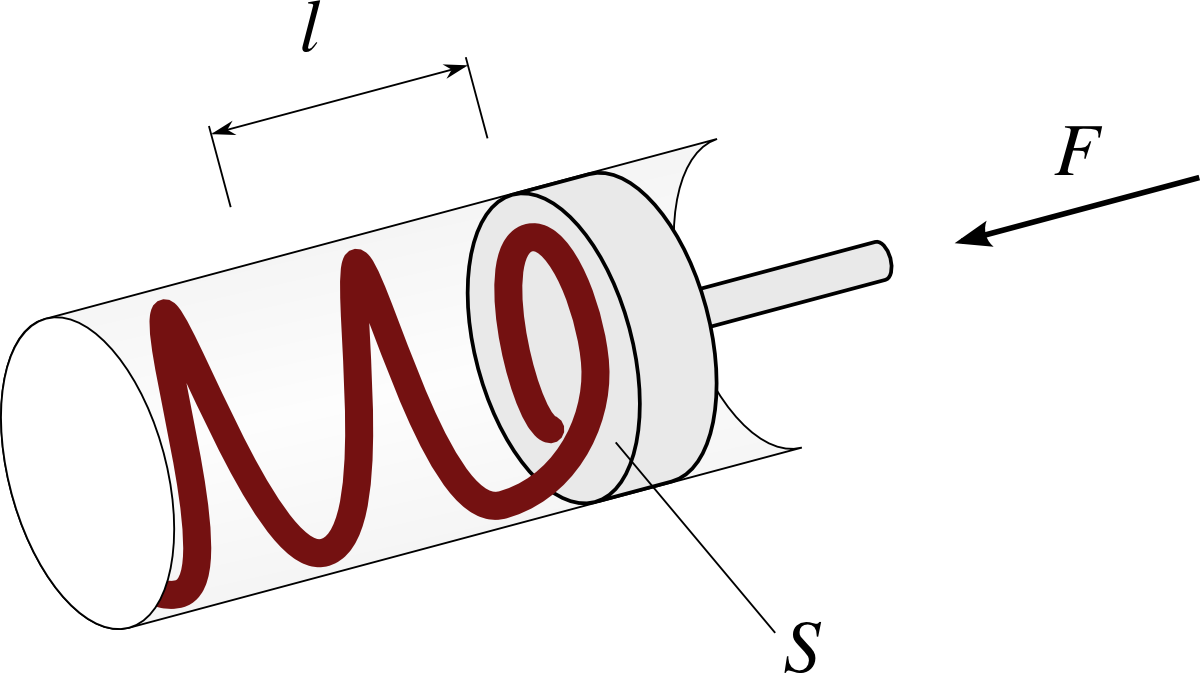
\includegraphics[width=12cm]{images/travail_cylindre_1.png}
			\end{center}
			\supercaption{Dans un premier temps, nous modélisons le fluide à l’intérieur du système avec un ressort métallique.}{schéma \ccbysa \olivier}
			\label{fig_piston_ressort}
		\end{figure}

		Commençons par imaginer que le fluide au sein d’un système fermé se comporte comme un ressort métallique (\cref{fig_piston_ressort}). C’est une modélisation intéressante pour débuter notre étude. Nous avions vu en \S\ref{ch_travail_fdl} que le travail fourni ou reçu par un ressort s’exprimait selon :
		\begin{equation*}
			W_\fromatob = - \int_\A^\B {F \diff l} \tag{\ref{eq_travail_fdl}}
		\end{equation*}

		Aujourd’hui, comme nous utilisons un fluide, nous voulons exprimer le travail en fonction des propriétés \vocab{pression} et \vocab{volume} plutôt que force et longueur.

		\clearfloats
		\begin{description}

			\item[La pression]{se définit comme une force divisée par une aire :
			\begin{equation}
				p \equiv \frac{F}{S}
				\label{def_pression}
			\end{equation}
			\begin{equationterms}
				\item où \tab $p$ \tab est la pression (\si{\pascal}),
				\item 	\tab $F$ \tab est la force (\si{\newton}),
				\item et \tab $S$ \tab est l’aire de la surface sur laquelle la force s’applique (\si{\metre\squared}).
			\end{equationterms}

			L’unité \textsc{si} de la pression est le~\si{Pascal},
			\begin{equation}
				\SI{1}{\pascal} \equiv \SI{1}{\newton\per\metre\squared}
			\end{equation}
			mais il est usuel d’utiliser le~\si{bar} pour unité :
			\begin{equation}
			\SI{1}{bar} \equiv \SI{1e5}{\pascal}
			\end{equation}

			Notons que la pression atmosphérique à faible altitude est de l’ordre du bar ($p_{\text{atm.std.}} \equiv \SI{1}{atm} \equiv \SI{1,01325}{bar}$). Attention, les manomètres indiquent parfois une pression jaugée, qui n’est pas la pression réelle. Cette différence est décrite dans l’annexe \ref{ch_annexe_pression}.
			}% end item

			\item[Le volume]{est également exprimable facilement. Si le système est déformé par un piston d’aire $S$, de sorte que sa longueur varie de $\diff l$, nous avons :
			\begin{equation}
			\diff V = S \diff l
			\label{eq_volume_surface_longueur}
			\end{equation}
			\begin{equationterms}
				\item où \tab $\diff V$ 	\tab est la variation infinitésimale du volume (\si{\metre\cubed}),
				\item 	\tab $S$ 			\tab\tab l’aire du piston déplacé (\si{\metre\squared}),
				\item et \tab $\diff l$ 	\tab\tab la variation infinitésimale de longueur du système correspondant au déplacement du piston (\si{\metre}).
			\end{equationterms}

			Dans le système d’unités \textsc{si} le volume se mesure en~\si{\metre\cubed} mais l’unité de mesure la plus courante est le~\si{litre} ($\SI{1}{\liter} \equiv \SI{e-3}{\metre\cubed})$.
			}% end item
		
		\end{description}


		Exprimons maintenant le travail d’un système fermé en fonction du volume et de la pression. En insérant les équations~\ref{def_pression} et~\ref{eq_volume_surface_longueur} dans l’\cref{eq_travail_fdl} nous obtenons :
		\begin{IEEEeqnarray}{rCl}
			W_\fromatob 	& = & - \int_\A^\B {F \diff l} = - \int_\A^\B {\frac{F}{S} S \diff l} 	\nonumber \\
			W_\fromatob 	& = & - \int_\A^\B {p \diff V} \label{eq_travail_pdV}
		\end{IEEEeqnarray}
		\begin{equationterms}
			\item pour un système fermé modélisé par un ressort,
			\item où \tab $W_\fromatob$ 	est le travail reçu par le système (\si{\joule}),
			\item 	\tab $p$ 				\tab\tab est la pression (homogène) intérieure (\si{\pascal}),
			\item et \tab $\diff V$ 		\tab la variation du volume (\si{\metre\cubed}).
		\end{equationterms}

		Pour pouvoir quantifier l’énergie stockée ou fournie par le système, il nous suffira donc de connaître la relation entre $p$ et $V$. Dans le cas présent, cette fonction $p_{(V)}$ est directement liée à la caractéristique $F_{(l)}$ du ressort. La dureté du ressort et sa géométrie (à spires régulières ou progressives) détermineront au final la quantité de travail stockée et fournie par le système.
		
		Un outil absolument formidable pour comprendre et analyser les transferts de chaleur est le \vocab{diagramme pression-volume}. Dans le cas où l’on modélise le fluide par un ressort, le travail peut être visualisé par l’aire sous la courbe d’une évolution (\cref{fig_p-v_ressort}).		

		\begin{figure}
			\begin{center}
				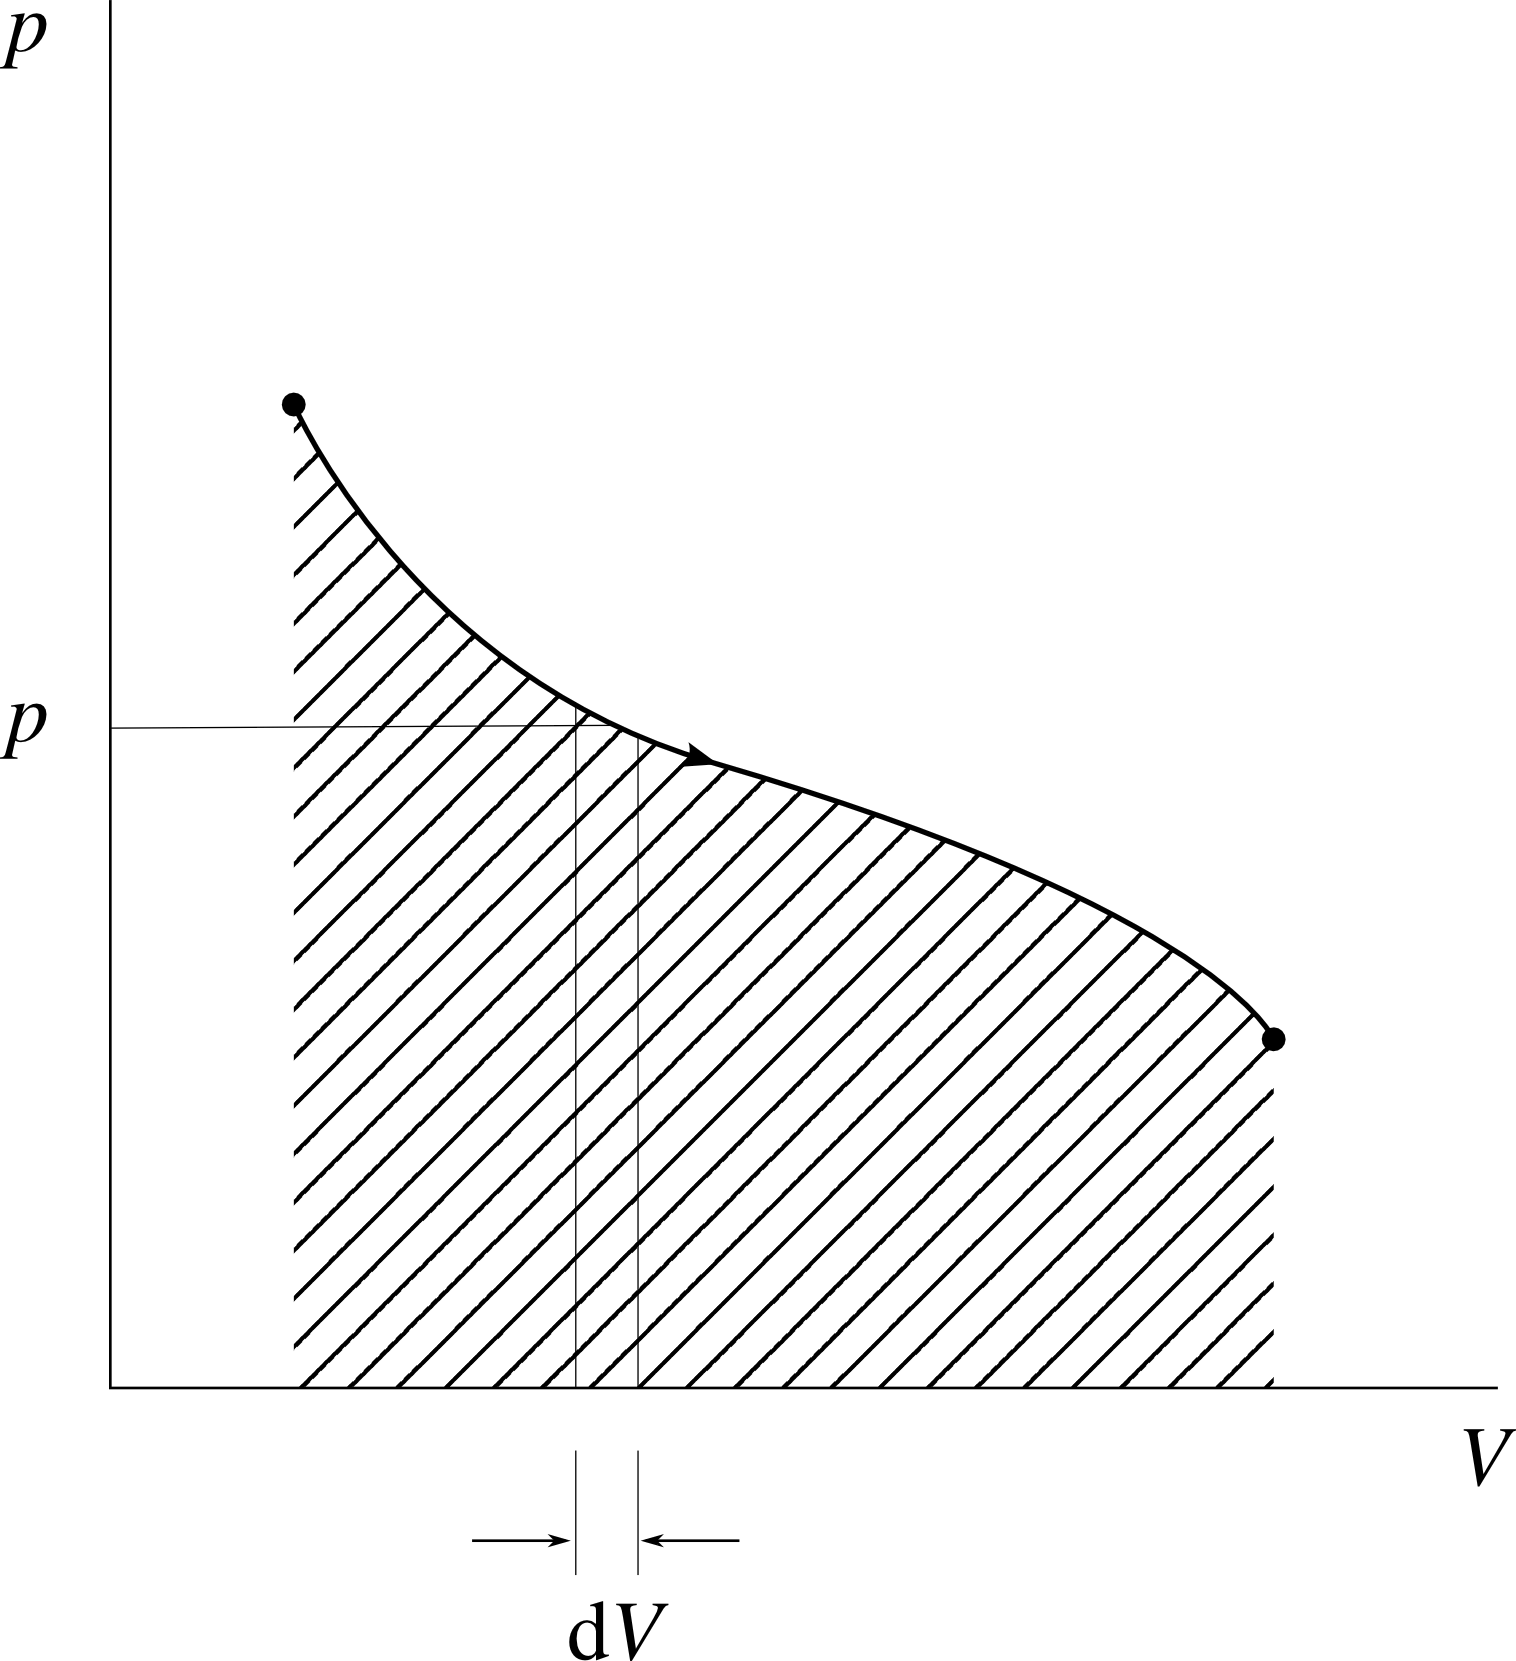
\includegraphics[width=8cm]{images/pv_ressort.png}
			\end{center}
			\supercaption{Diagramme pression-volume d’un système fermé modélisé par un ressort. Dans le cas représenté, le volume augmente (le piston s’éloigne). La grandeur $\diff V$ sera constamment positive, et le travail sera négatif : le système perd de l’énergie au profit du piston.\\
			Cette figure représente le même phénomène qu’en \cref{fig_force-déplacement-aire} avec des grandeurs différentes.}{}
			\label{fig_p-v_ressort}
		\end{figure}

		\begin{anexample}
			
			Un système fermé est constitué d’une boîte vide dans laquelle on a placé un ressort. La pression exercée par le ressort sur les parois de la boîte est constante à $p = \SI{e5}{\pascal}$ quelque soit son volume. On comprime la boîte depuis un volume $V_\A = \SI{2}{\liter}$ jusqu’à $V_\B = \SI{1}{\liter}$. Quel est le transfert de travail ?
				\begin{answer}
						Sur un diagramme pression-volume et de façon qualitative (c’est-à-dire sans représenter les valeurs numériques), l’évolution peut être représentée ainsi :
							\begin{center}
								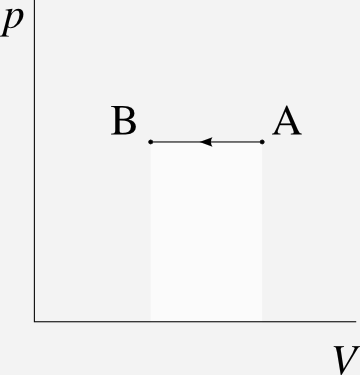
\includegraphics[width=3cm]{images/exe_pv_isobare.png}
							\end{center}
					Nous partons de l’équation \ref{eq_travail_pdV} : $W_{\A\to\B} = - \int_\A^\B p \diff V = - p_\text{cste.} \int_\A^\B \diff V = p_\text{cste.} \left[V\right]_{V_\A}^{V_\B } = - \num{e5} (\num{1e-3} - \num{2e-3}) = \SI{+100}{\joule}.$
					\begin{remark}Le signe est positif : la boîte («~le système~») reçoit du travail. Nous explicitons toujours le signe en quantifiant les transferts.\end{remark}
				\end{answer}
		\end{anexample}


		\begin{anexample}
			Un système fermé a une pression interne liée à son volume par la relation $p = \num{7e5} - \num{2e8} \ V$ (en unités \textsc{si}). On comprime la boîte depuis un volume $V_\A = \SI{2}{\liter}$ jusqu’à $V_\B = \SI{1}{\liter}$. Combien a-t-il reçu ou perdu d’énergie sous forme de travail ?
				\begin{answer}
						Sur un diagramme pression-volume et de façon qualitative, l’évolution peut être représentée ainsi :
							\begin{center}
								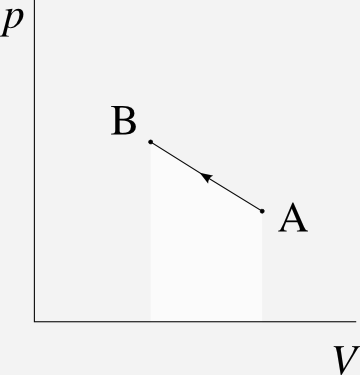
\includegraphics[width=3cm]{images/exe_pv_prop.png}
							\end{center}
					Encore une fois nous partons de l’\cref{eq_travail_pdV} : $W_{\A\to\B} = - \int_\A^\B p \diff V = - \int_\A^\B (\num{7e5} - \num{2e8} V) \diff V = - \left[\num{7e5}V - \frac{1}{2}\num{2e8} V^2\right]_{V_\A}^{V_\B } = - (\num{700} - 100 - \num{1400} + 400) = \SI{+400}{\joule}$ (positif : travail reçu par le système).
				\end{answer}
		\end{anexample}
		

	\subsection{Travail d’un fluide en évolution lente}

		Lorsque l’on comprime un fluide, les molécules qui le composent sont plus rapprochées les unes des autres (\cref{fig_molécules_compression_lente}) et les collisions entre elles et contre les parois deviennent plus fréquentes. À l’échelle macroscopique, cette augmentation se traduit par une augmentation de la pression.
		
		\begin{figure}
			\begin{center}
			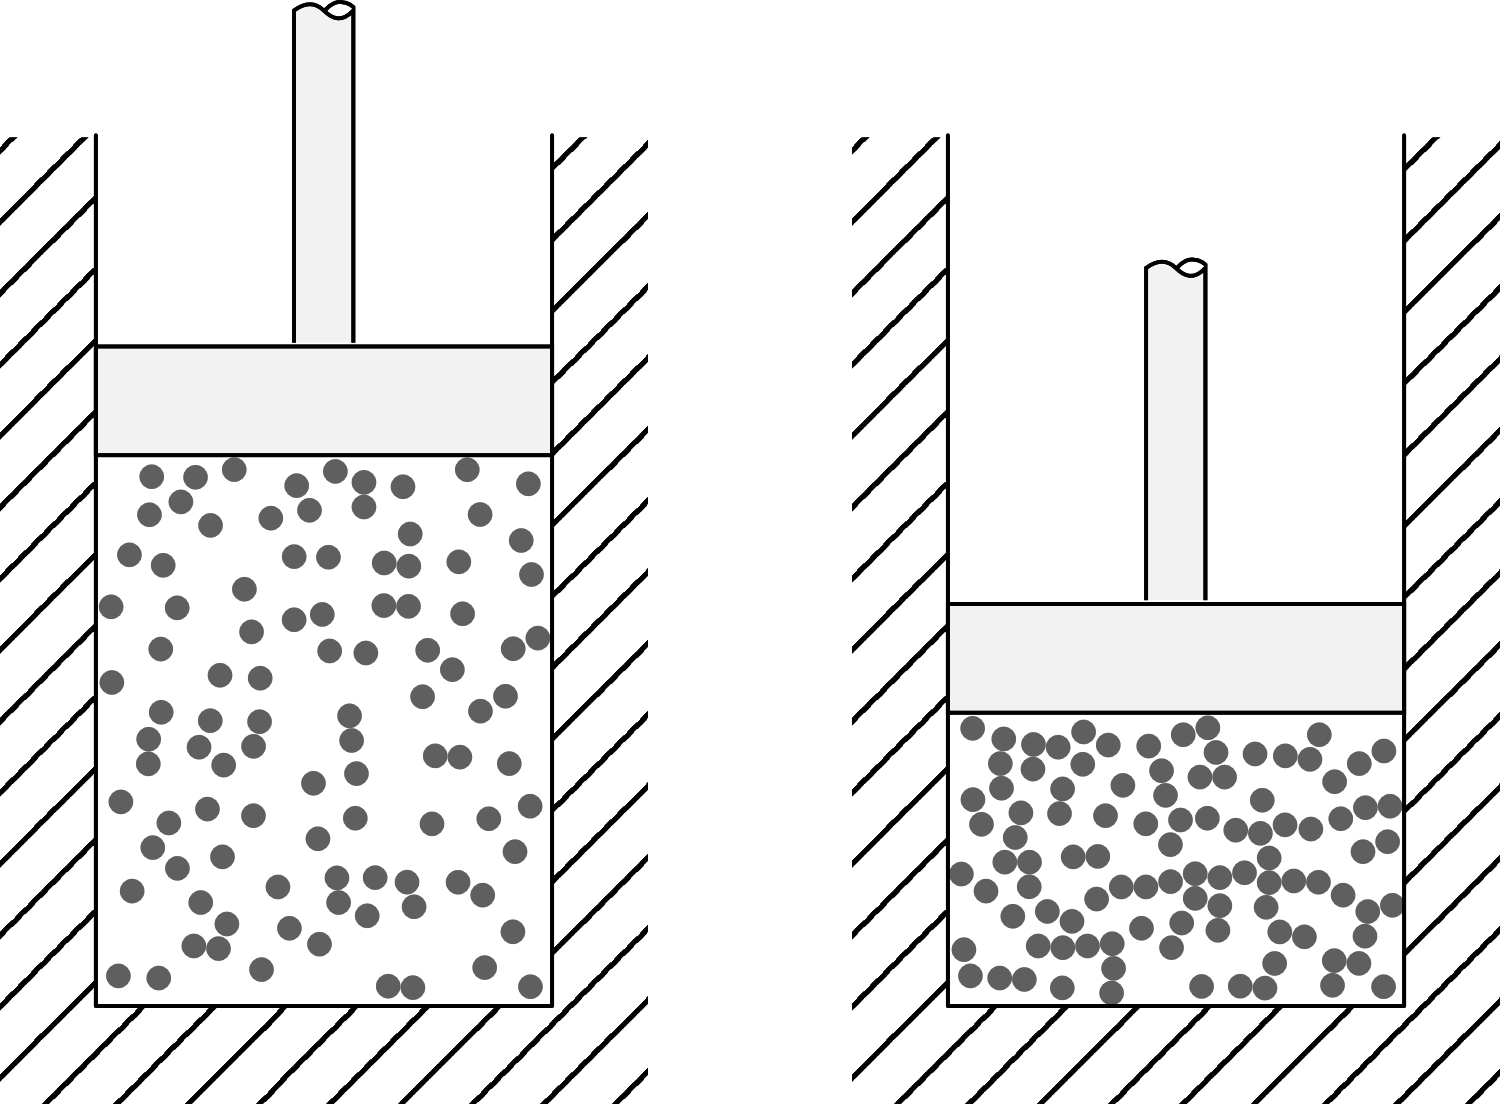
\includegraphics[width=9cm]{images/particules_compression_lente.png}
			\end{center}
			\supercaption{Une représentation simpliste d’un fluide que l’on \mbox{comprime} infiniment lentement sans le chauffer. Le fluide voit sa température et sa pression augmenter.}{schéma \cczero \oc}
			\label{fig_molécules_compression_lente}
		\end{figure}

		Nous constatons expérimentalement que lorsque le mouvement est infiniment lent, un fluide comprimé se comporte exactement comme un ressort (\cref{fig_piston_fluide_lent}). La précision «~lorsque le mouvement est infiniment lent~» est d’importance capitale, comme nous le verrons plus bas.

		\begin{figure}
			\begin{center}
			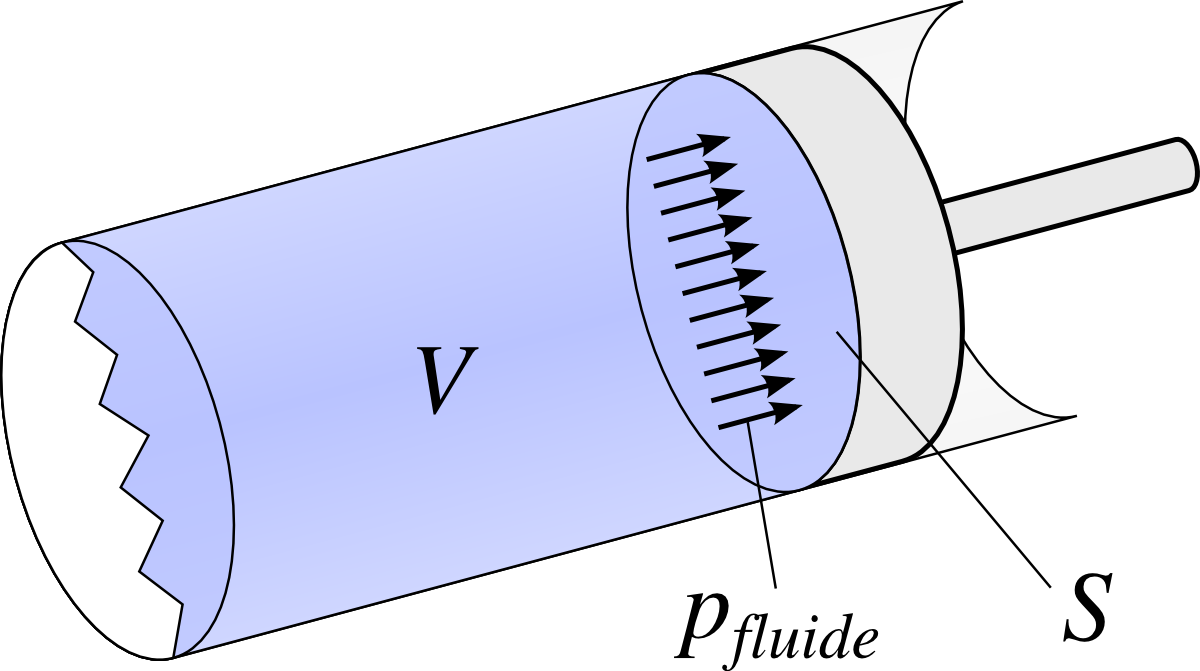
\includegraphics[width=10cm]{images/travail_cylindre_2.png}
			\end{center}
			\supercaption{Lorsque le mouvement du piston est infiniment lent, le fluide se comporte comme un ressort que l’on comprime.}{schéma \ccbysa \olivier}
			\label{fig_piston_fluide_lent}
		\end{figure}

		
		Si cette condition est respectée, nous pouvons exprimer le travail reçu ou perdu par le système de la même façon qu’avec le ressort de la section précédente :		
		\begin{IEEEeqnarray}{rCl}
			W_\fromatob 	& = & - \int_\A^\B {p \diff V}	\nonumber \\
			w_\fromatob 	& = & - \int_\A^\B p \diff v
			\label{eq_travail_pdv}
		\end{IEEEeqnarray}
		\begin{equationterms}
			\item pour un système fermé lorsque les variations de volume sont infiniment lentes ;
			\item où \tab $w_\fromatob$ 	\tab est le travail spécifique reçu par le système (\si{\joule\per\kilogram}),
			\item 	\tab $p$ 				\tab\tab est la pression (homogène) intérieure (\si{\pascal}),
			\item et \onlyamphibook{\tab} $\diff v $ 		\onlyamphibook{\tab} la variation du volume spécifique (\si{\metre\cubed\per\kilogram}). % floating quote messes with the tabs in Framabook, so they are commented out here.
		\end{equationterms}
		
		\thermoquotebegin{O}
			Cela posé, prenons un gaz quelconque à la température $T$ […]; représentons son volume $v_o$ par l’abscisse \textsc{ab}, et sa pression par l’ordonnée \textsc{cb}.[…] Le gaz, pendant sa dilatation, aura développé une quantité d’action mécanique qui aura pour valeur l’intégrale du produit de la pression, par la différentielle du volume, et qui sera représentée géométriquement par la surface comprise entre l’axe des abscisses, les deux coordonnées \textsc{cb}, \textsc{de}, et de la portion d’hyperbole~\textsc{ce}.
		\thermoquoteend{Benoît Paul Émile Clapeyron, 1834\\ {\tiny(le premier diagramme $p-v$…)}}{\textit{Mémoire sur la puissance motrice de~la~chaleur}~\cite{clapeyron1834}\vspace{6em}} %handmade vspace
		Sur un graphique représentant la pression en fonction du volume spécifique, ce travail $w_\fromatob$ est représenté par la surface sous la courbe de A à B, exactement comme la \cref{fig_p-v_ressort}. La forme de la courbe, c’est-à-dire la relation entre $p$ et $v$ au fur et à mesure de l’évolution, déterminera la quantité $w_\fromatob$ .

		\begin{figure}
			\begin{center}
			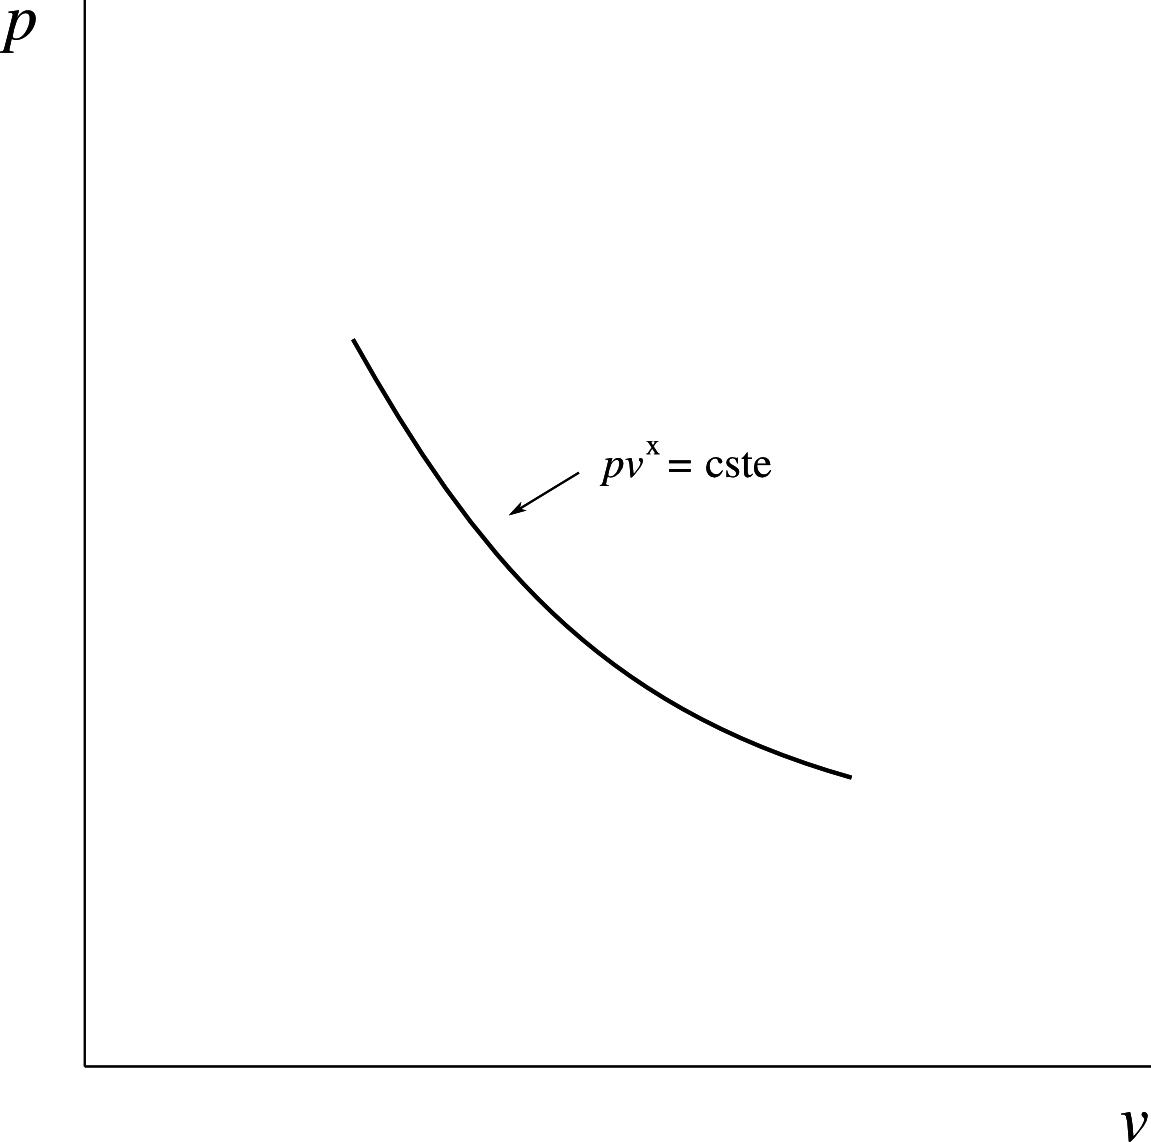
\includegraphics[width=\pvdiagramwidth]{images/pv_gaz_simple.png}
			\end{center}
			\supercaption{Propriétés d’un gaz lorsqu’on le comprime. La relation est similaire à celle que l’on obtiendrait avec un ressort à spires progressives.}{schéma \cczero \oc}
			\label{fig_p-v_pvx}
		\end{figure}

		\thermoquotebegin{O}
			S’il était vrai que la vapeur se dépensât par le cylindre à une pression égale à celle de la chaudière, ou qui fût à celle-ci dans un rapport fixe indiqué par un coefficient quelconque, puisqu’il faut toujours à une même locomotive le même nombre de tours de roue, ou le même nombre de coups de piston pour parcourir la même distance, il s’en suivrait que tant que ces machines travaillent à la même pression, elles devraient consommer dans tous les cas la même quantité d’eau pour la même distance.
		\thermoquoteend{François-Marie Guyonneau de~Pambour, 1839}{\textit{Théorie de la machine à vapeur} \cite{pambour1839}\vspace{4em}} %handmade vspace
		Comment les fluides se comportent-t-ils lorsqu’on les comprime --\ autrement dit, par quel type de «~ressort~» peut-on les modéliser ? On constate expérimentalement que, lorsqu’on les comprime, la plupart des gaz voient leur pression et leur volume liés par une relation de type $p\ v^{x} = \text{cste.}$ avec $x$ une constante lorsqu’on les comprime (\cref{fig_p-v_pvx})%
			\footnote{Toutefois, nous verrons au \courscinqshort que les liquides/vapeurs ne se comportent pas du tout comme cela sur une plage de propriétés donnée, même si la tendance globale reste la même.}%
		.

		Lorsqu’on apporte de la chaleur au fluide pendant qu’on le comprime, on «~durcit~» son comportement, et la pression augmente plus rapidement (\cref{fig_p-v_ajout_retrait_chaleur}). À~l’inverse, lorsqu’on lui prélève de la chaleur pendant la compression, la pression augmente moins rapidement. Ces transferts de chaleur font donc varier la quantité de travail à fournir pour comprimer le fluide entre deux volumes donnés.
		
		Le cas où l’on apporte pas de chaleur est nommé \vocab{adiabatique} : $Q = 0$. Attention : adiabatique ne veut pas dire «~à température constante~». Lorsque l’on comprime un fluide sans apport de chaleur, sa température augmente. Dans un moteur diesel, par exemple, l’air dans les cylindres peut atteindre \SI{900}{\degreeCelsius} avant la combustion -- ce qui est désirable, comme nous le verrons au \courssept.

		\begin{figure}
			\begin{center}
			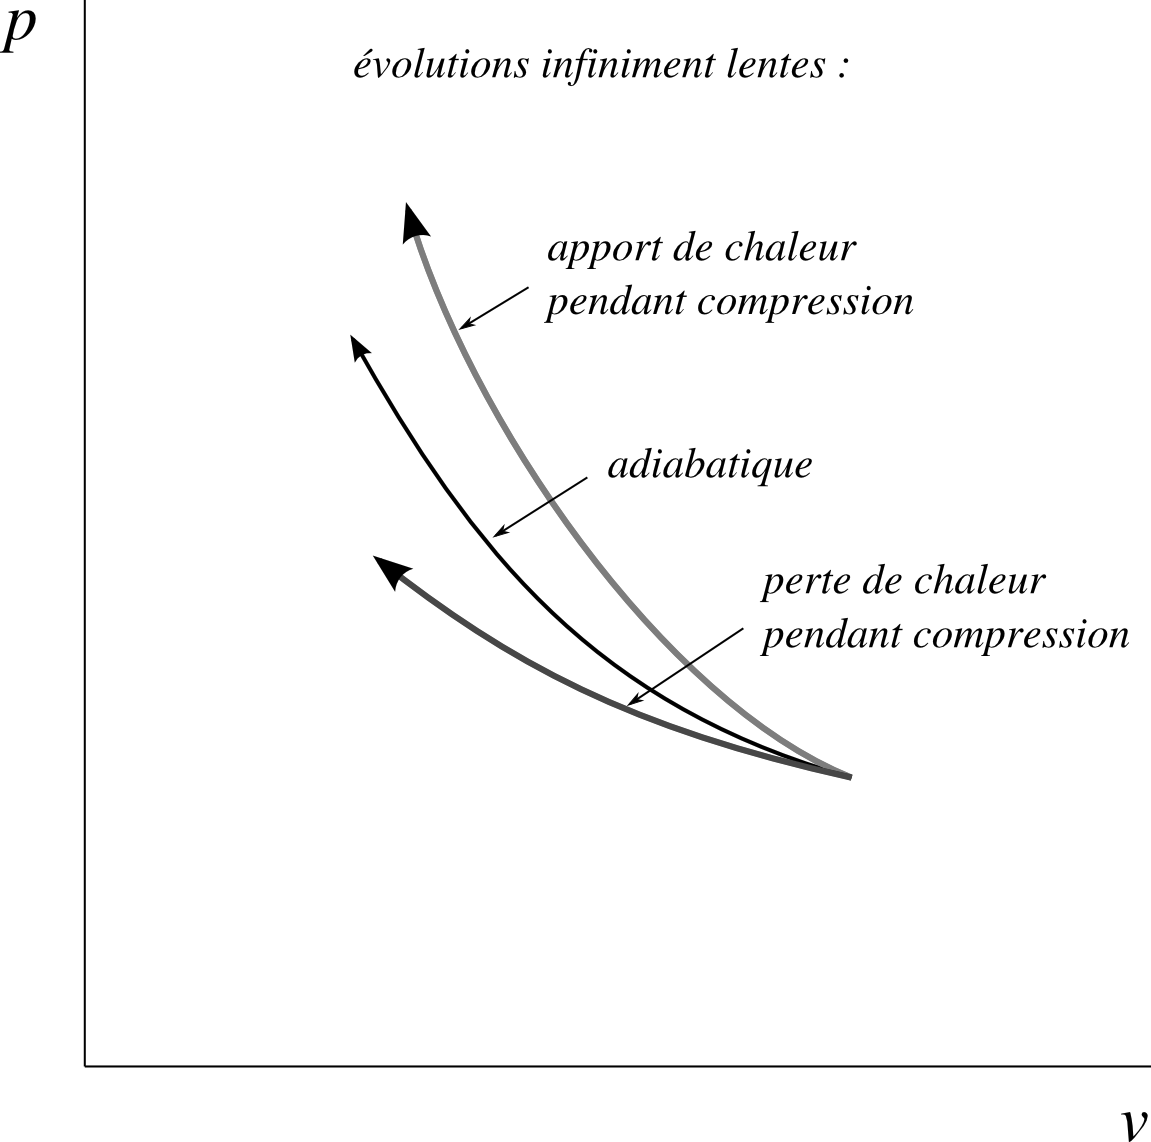
\includegraphics[width=\didacticpvdiagramwidth]{images/pv_transfert_chaleur.png}
			\end{center}
			\supercaption{Comportement d’un fluide lorsqu’on le comprime infiniment lentement.
Plus on lui apporte de chaleur pendant la compression, plus la pression augmente fortement. La courbe adiabatique représente le cas où aucun apport ni perte de chaleur n’a lieu ($Q = 0$).}{schéma \cczero \oc}
			\label{fig_p-v_ajout_retrait_chaleur}
		\end{figure}


		Dans les trois évolutions de la \cref{fig_p-v_ajout_retrait_chaleur}, la relation de type $p v^{x} = \text{cste.}$ reste une modélisation appropriée. Plus on apporte de chaleur pendant la compression, plus la pression augmente rapidement --\ l’exposant $x$ est alors plus important.

		Inversement, si l’on prélève de la chaleur pendant la compression, la pression augmente moins rapidement et on obtient une courbe plus proche de l’horizontale (avec un exposant $x$ plus faible). En prélevant suffisamment de chaleur, on peut même maintenir la pression constante, comme nous le verrons aux chapitres~\quatre et~\cinq. L’exposant $x$ est alors nul et on a $p = p_\text{cste.}$.
		
			\begin{anexample}
				Un gaz dans un cylindre est comprimé lentement par un piston. On observe que sa pression est liée à son volume par la relation $p v^{\num{1,2}} = k$ (en unités \textsc{si}, et où $k$ est une constante). Au début de la compression, ses propriétés sont $p_\A = \SI{1}{\bar}$ et $v_\A = \SI{1}{\metre\cubed\per\kilogram}$. On le comprime jusqu’à ce que son volume ait atteint $v_\B = \SI{0,167}{\metre\cubed\per\kilogram}$. \\
				Quelle quantité de travail spécifique le gaz a-t-il fourni ou reçu ?				
					\begin{answer}
						Sur un diagramme pression-volume et de façon qualitative, l’évolution peut être représentée ainsi :
							\begin{center}
								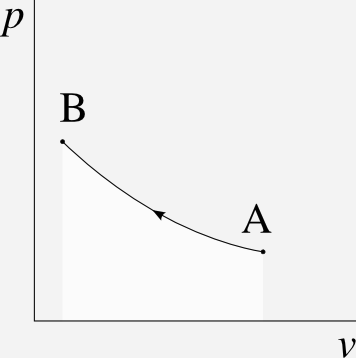
\includegraphics[width=3cm]{images/exe_pv_exp1.png}
							\end{center}
						Il nous faut d’abord calculer la valeur de $k$ pour connaître quantitativement la relation entre $p$ et $v$. Nous l’obtenons avec les conditions initiales : $k = p_\A v_\A^{\num{1,2}} = \num{e5} \times 1^{\num{1,2}} = \SI{e5}{\usi}$.
							\begin{remark} La grandeur de $k$ est déroutante : elle est mesurée en~\si{\pascal\metre\tothe{3,6}\per\kilogram\tothe{1,2}}. Cela n’a pas d’importance pour nous et il nous suffit (après avoir bien converti les unités d’entrée en \textsc{si}!) d’indiquer «~unités \textsc{si}~», ou~\si{\usi}.\end{remark}
						Maintenant, nous pouvons décrire $p$ en fonction de $v$ : $p = \num{e5} \times v^{\num{-1,2}}$. Il n’y a plus qu’à intégrer en partant de l’\cref{eq_travail_pdv} : $w_\fromatob = - \int_\A^\B p \diff v = - \int_\A^\B k v^{\num{-1,2}} \diff v = - k \left[\frac{1}{-1,2 + 1} v^{-1,2 - 1} \right]_{v_\A}^{v_\B } = \frac{\num{e5}}{0,2}\left[v^{-0,2}\right]_1^{\num{0,167}} = \SI{+2,152e5}{\joule\per\kilogram} = \SI{+215,2}{\kilo\joule\per\kilogram}$.
							\begin{remark}Le signe est positif : le gaz reçoit du travail.\end{remark}
							\begin{remark}Le résultat peut paraître grand, mais il faut se rappeler que c’est un travail spécifique (\S\ref{ch_valeurs_spécifiques}) qu’il faudra multiplier par la masse du gaz pour obtenir une quantité en joules. Aux conditions de départ (\SI{1}{\kilogram\per\metre\cubed}) un volume d’air de~\SI{1}{\liter} pèse à peine plus d’un~\si{gramme}. \end{remark}
					\end{answer}
			\end{anexample}

			\begin{anexample}
				Une masse de~\SI{0,3}{gramme} de gaz pressurisée dans un cylindre est détendue lentement en laissant un piston se déplacer. On sait que sa pression et son volume sont reliés par une relation de type $p v^{k_1} = k_2$ (où $k_1$ et $k_2$ sont deux constantes).\\
				Au début de la détente, la pression est à~\SI{12}{\bar} et le volume est de~\SI{0,25}{\liter}. Une fois détendu, le gaz arrive à pression ambiante de~\SI{1}{\bar} avec un volume de~\SI{1,76}{\liter}.\\
				Quel travail le gaz a-t-il dégagé pendant la détente ?				
					\begin{answer}
						Sur un diagramme pression-volume et de façon qualitative, l’évolution peut être représentée ainsi :
							\begin{center}
								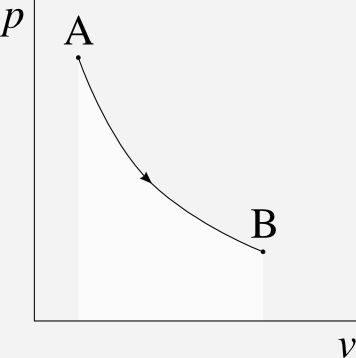
\includegraphics[width=3cm]{images/exe_pv_exp2.png}
							\end{center}
						Il nous faut d’abord connaître entièrement la loi reliant $p$ à $v$ ; ensuite nous procéderons à l’intégration $-\int p \diff v$ pendant l’évolution pour calculer le travail.\\
						Commençons par calculer les volumes spécifiques au départ et à l’arrivée : $v_\A = \frac{V_\A}{m} = \frac{\num{0,25e-3}}{\num{3e-4}} = \SI{0,833}{\metre\cubed\per\kilogram}$. De même, $v_\B = \frac{V_\B }{m} = \SI{5,867}{\metre\cubed\per\kilogram}$.
						Maintenant, nous pouvons calculer $k_1$ :		
							\begin{IEEEeqnarray*}{rCl}
								p_\A v_\A^{k_1} 	&=& p_\B v_\B ^{k_1}	\\
								\left(\frac{v_\A}{v_\B }\right)^{k_1} &=& \frac{p_\B }{p_\A}\\
								k_1 \ln\left(\frac{v_\A}{v_\B }\right) &=& \ln \left(\frac{p_\B }{p_\A}\right)\\
								k_1 &=& \frac{\ln\left(\frac{p_\B }{p_\A}\right)}{\ln\left(\frac{v_\A}{v_\B }\right)} = \frac{\ln\left(\frac{1}{12}\right)}{\ln\left(\frac{0,833}{5,867}\right)} = \num{1,2733}
							\end{IEEEeqnarray*}
						Et avec $k_1$, nous pouvons calculer $k_2 = p_\A v_\A^{k_1} = \num{12e5} \times \num{0,833}^{\num{1,2733}} = \SI{9,514e5}{\usi}$.
							\begin{remark}$k_1$ est un exposant et n’a pas d’unités. Les unités de $k_2$ ne nous intéressent pas.\end{remark}
							\begin{remark}Même si elle peut paraître laborieuse, cette démarche «~nous avons un modèle général pour la tendance, quels sont les paramètres pour ce cas particulier ?~» est très courante en physique, et extrêmement utile pour l’ingénieur/e.\end{remark}
						Nous savons maintenant décrire quantitativement les propriétés pendant l’évolution : $p v^{\num{1,2733}} = \num{5,914e5}$.	Il n’y a plus qu’à effectuer notre intégration habituelle : $w_\fromatob = - \int_\A^\B p \diff v = - k_2 \int_\A^\B v^{-k_1} \diff v = \frac{\num{-9,514e5}}{\num{-0,2733}} \left[v^{-0,2733}\right]_{\num{0,833}}^{\num{0,587}} = \SI{-3,333e6}{\joule\per\kilogram} = \SI{-3333}{\kilo\joule\per\kilogram}$. Nous multiplions par la masse de gaz pour obtenir le travail : $W_{\A\to\B} = m \ w_\fromatob = \SI{-1}{\kilo\joule}$.
							\begin{remark}Ce calcul peut être effectué de façon plus rapide, sans calculer les valeurs de $v_\A$, $v_\B $ et $k_2$. Toutefois, pour être certain/e de parvenir au résultat, il est plus sûr et plus facile de quantifier $p$ et $v$ (en \textsc{si}) à tous les stades de l’évolution avant de débuter une intégration.\end{remark}
					\end{answer}
			\end{anexample}
			
			\begin{anexample}
				Un gaz enfermé dans un réservoir hermétique est chauffé lentement. Son volume reste bloqué à~\SI{12}{\liter}, et sa pression évolue de~\SI{1}{\bar} jusqu’à \SI{40}{\bar}. Quel est le travail développé ?
					\begin{answer}
						Sur un diagramme pression-volume et de façon qualitative, l’évolution peut être représentée ainsi :
							\begin{center}
								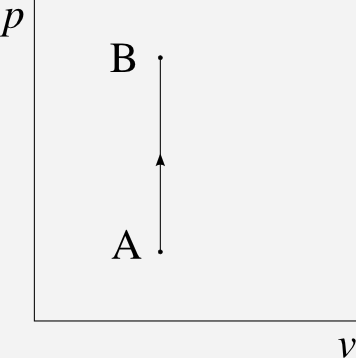
\includegraphics[width=3cm]{images/exe_pv_isochore.png}
							\end{center}
						Le travail est nul, bien sûr. Le volume ne changeant pas, $\diff V$ est nul pendant toute l’évolution. Nous pouvons chauffer ou refroidir à loisir, mais tant qu’aucune paroi n’est déplacée, il n’y aura pas de transfert de travail.
					\end{answer}
			\end{anexample}
			

	\subsection{Travail d’un fluide en évolution rapide}
	\label{ch_évolutions_irr_sf}

		\thermoquotebegin{O}
			Nous avons dit qu’à l’origine du mouvement l’équilibre de pression s’établit entre la chaudière et le cylindre, mais à mesure que la vitesse du piston s’accroît, celui-ci fuit en quelque sorte devant la vapeur sans lui donner le temps d’établir cet équilibre, et la pression dans le cylindre baisse \mbox{nécessairement}.
		\thermoquoteend{François-Marie Guyonneau de~Pambour, 1835}{\textit{Traité théorique et pratique des machines locomotives}~\cite{pambour1835}\vspace{3em}} %handmade vspace
		Les choses se compliquent lorsque nous comprimons et détendons notre fluide de façon rapide (\cref{fig_molécules_rapide}). Il se produit alors un phénomène complexe et d’importance critique en thermodynamique : \textbf{la pression sur la paroi est différente de la «~pression moyenne~» à l’intérieur du fluide}.

		\begin{figure}
			\begin{center}
			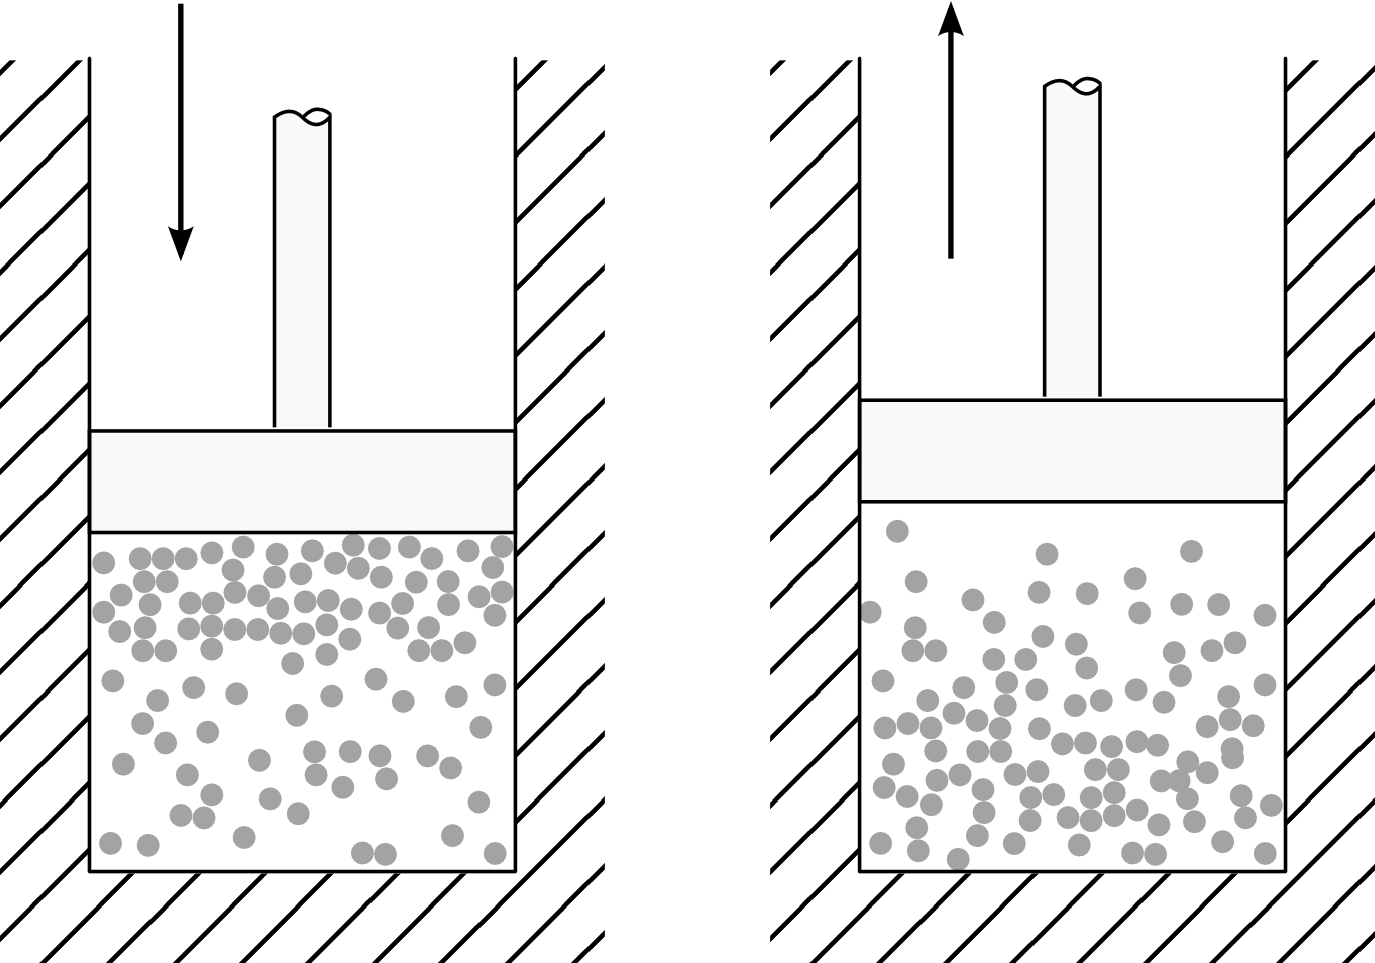
\includegraphics[width=9cm]{images/particules_compression_rapide.png}
			\end{center}
			\supercaption{Compression et détente irréversibles. Lorsqu’on comprime un fluide de façon brutale (schéma de gauche), la pression sur la paroi du piston est augmentée. Lors d’une détente brutale (schéma de droite) cette pression est diminuée.}{schéma \ccbysa \olivier}
			\label{fig_molécules_rapide}
		\end{figure}

		Pour décrire ce qui se passe à l’intérieur du fluide, nous pouvons prendre l’exemple de l’eau d’une baignoire que l’on pousse avec les mains --\ comme la paroi mobile dans le réservoir représenté en \cref{fig_baignoire}. Lorsque le piston est éloigné et rapproché brutalement, la pression sur ses parois n’est pas la même que lorsqu’il est déplacé lentement.

		\begin{figure}[htb!]%handmade: Là il faut poser les figures avant de continuer, sinon ça devient trop dur à suivre.
			\begin{center}
				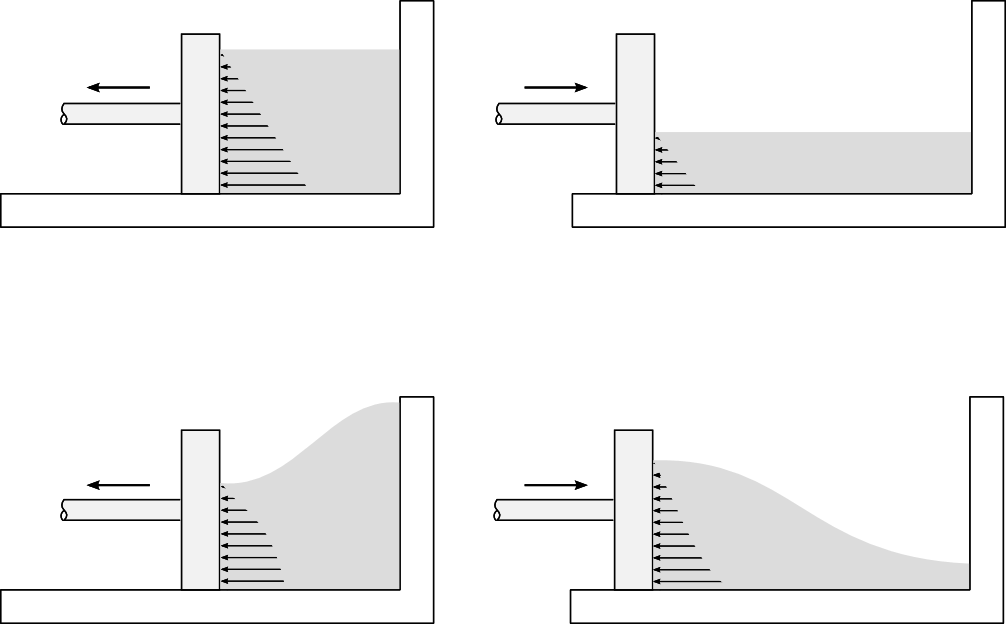
\includegraphics[width=\textwidth]{images/mouvement_rapide_niveau_eau.png}
			\end{center}
			\supercaption{Paroi mobile déplaçant une masse d’eau dans un réservoir : en haut, selon un mouvement infiniment lent ; en bas, avec un mouvement brutal. Les flèches représentent la pression appliquée sur la paroi mobile par l’eau.}{schéma \cczero \oc}%FIXME : vérifier seuil d’originalité, cette figure est repiquée de Çengel & al 2007
			\label{fig_baignoire}
		\end{figure}
		
		Dans chacun des cas, la quantité de travail consommé à la compression est plus grande et la quantité de travail fourni à la détente est plus petite.
		
		Nous nommons ce phénomène l’\vocab{irréversibilité}. Elle nous sera d’un grand embarras dans notre étude quantitative de la thermodynamique et elle rendra encore plus ardues nos conversions de travail et chaleur.

		Que se passe-t-il donc dans le cylindre empli de fluide, lorsqu’on ne le comprime pas de façon infiniment lente ? Lors d’une compression brutale, la pression sur la paroi du piston est plus grande que la pression moyenne à l’intérieur du cylindre (\cref{fig_piston_fluide_rapide}). On dépense \emph{plus d’énergie que nécessaire} pour effectuer le déplacement.

		\begin{figure}
			\begin{center}
				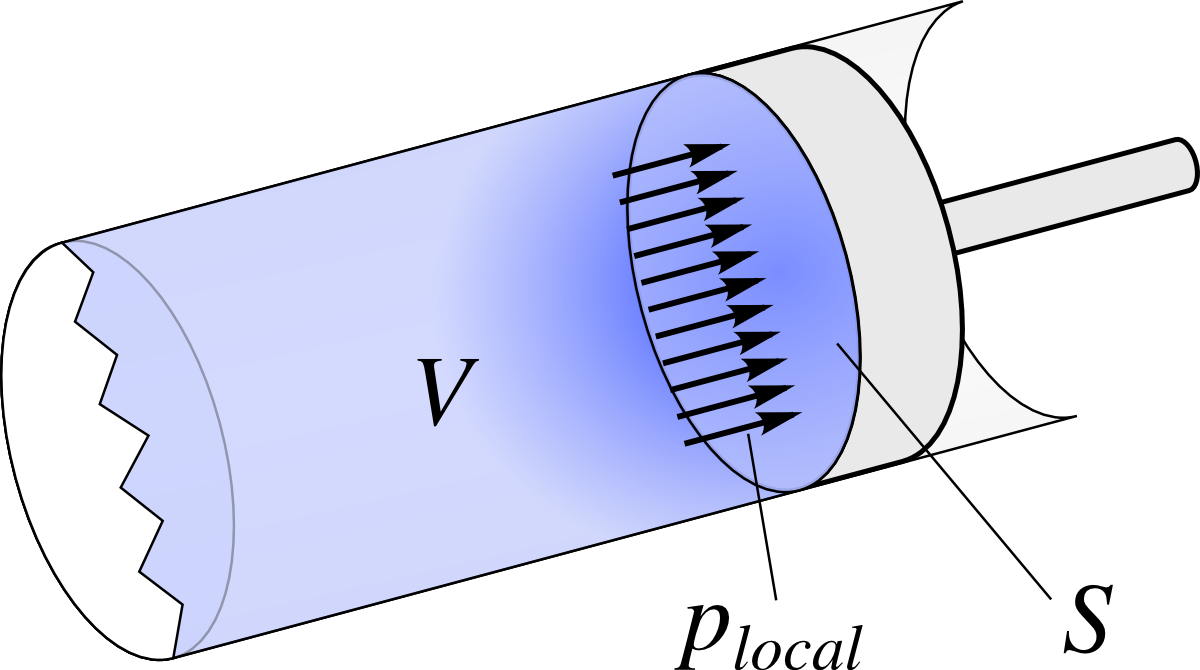
\includegraphics[width=10cm]{images/travail_cylindre_3.png}
			\end{center}
			\supercaption{Fluide comprimé de façon brutale. La pression locale à la surface du piston est supérieure à ce qu’elle aurait été avec un mouvement lent.}{schéma \ccbysa \olivier}
			\label{fig_piston_fluide_rapide}
		\end{figure}

		On pourrait ainsi dire que lorsqu’on le comprime et détend brutalement, un fluide se comporte comme un ressort «~fragile~», à l’intérieur duquel quelque chose se modifie : il n’est pas capable de rendre toute l’énergie mécanique qu’il a emmagasinée.

		Si le travail reçu n’est pas égal au travail restitué, alors où est passé l’excédent d’énergie ? Ce surcroît d’énergie, fourni sous forme de travail par le piston, est \emph{transformé en chaleur à l’intérieur du fluide} pendant les mouvements.

		\clearfloats % encore une fois, sinon c’est trop b****lique

		L’évolution tracée sur un diagramme pression-volume (\cref{fig_p-v_compression_irr}) est bien plus complexe que dans le cas d’une évolution infiniment lente. La pression moyenne à l’intérieur du fluide augmente plus rapidement qu’elle ne le ferait en mouvement lent.

		\begin{figure}
			\begin{center}
				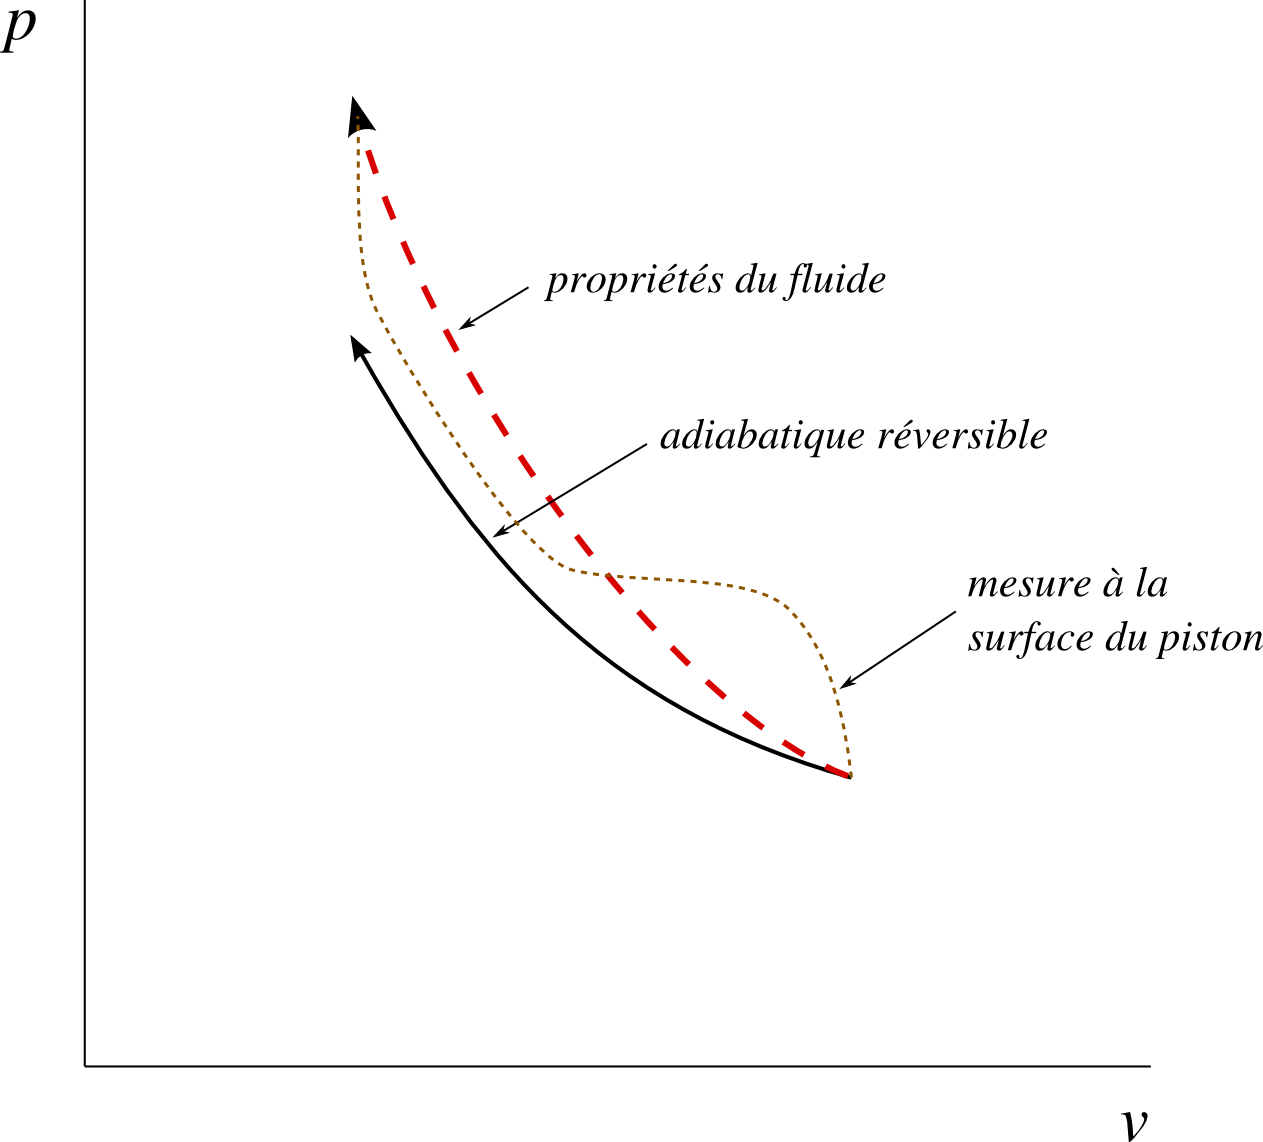
\includegraphics[width=\didacticpvdiagramwidth]{images/pv_compression_irreversible.png}
			\end{center}
			\supercaption{Compression irréversible adiabatique sur un diagramme pression-volume.\\
				Nous représentons l’évolution du gaz en pointillés : il ne s’agit pas d’une série d’états continue car la pression du fluide n’est pas homogène pendant le trajet.\\
				Le chemin qu’aurait suivi le fluide si la compression avait été infiniment lente est représenté avec un trait continu.\\
				Pendant la compression, le «~surcoût~» de travail fourni par le piston est transformé en chaleur (bien que le gaz soit parfaitement isolé).}{schéma \cczero \oc}
			\label{fig_p-v_compression_irr}
		\end{figure}

		Pendant la détente, le phénomène inverse se produit (\cref{fig_p-v_détente_irr}) : une zone de plus faible pression se forme au devant de la paroi du piston, et le travail fourni par le fluide au piston est plus faible qu’il ne l’aurait été dans le cas réversible.

		\begin{figure}
			\begin{center}
			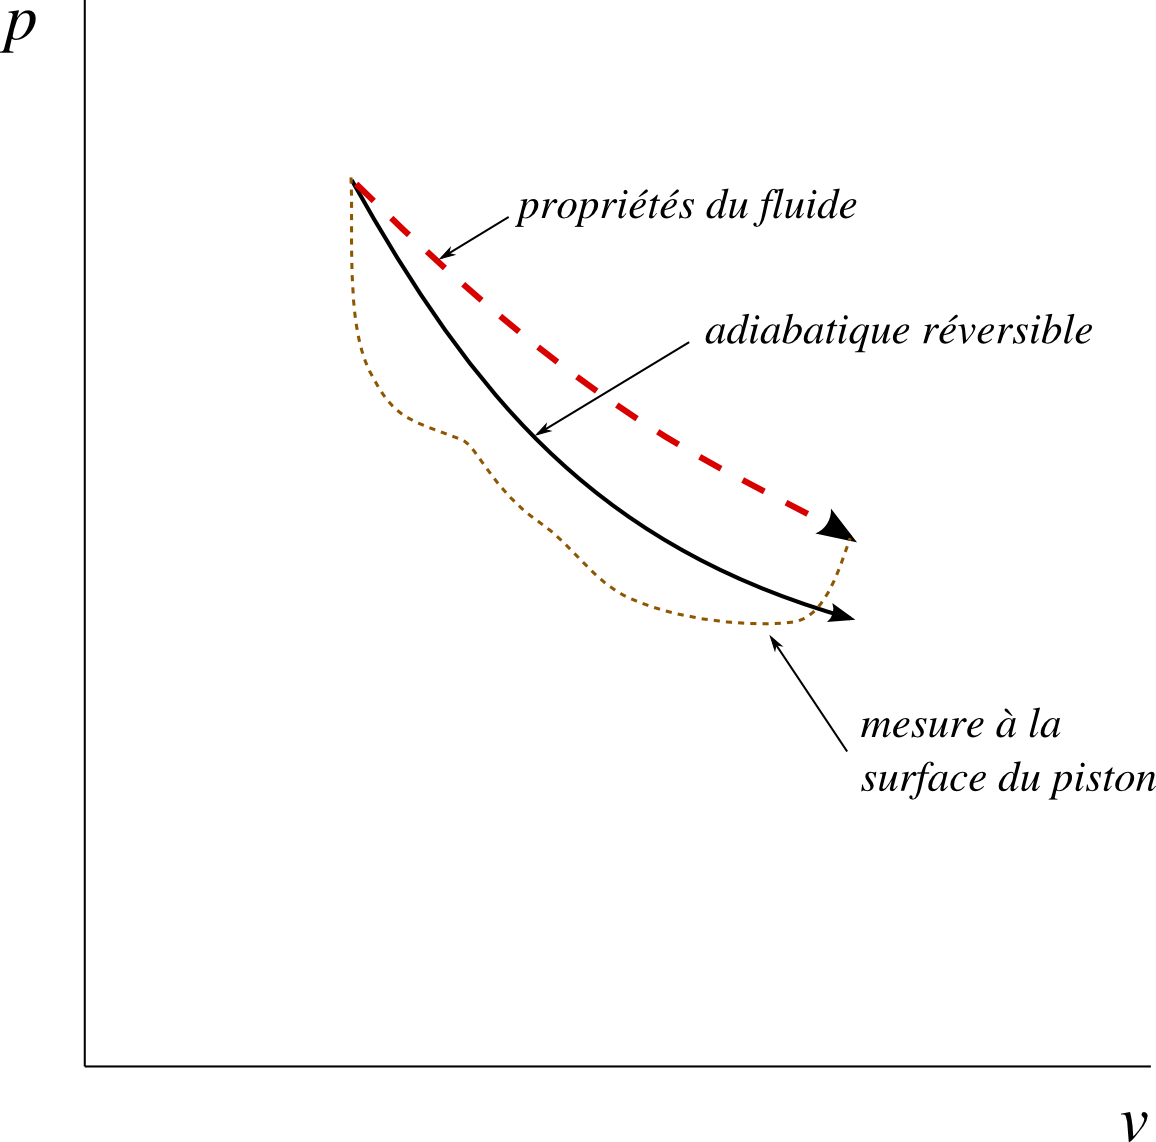
\includegraphics[width=9cm]{images/pv_detente_irreversible.png}
			\end{center}
			\supercaption{Détente irréversible adiabatique sur un diagramme pression-volume.\\ Le travail reçu par le piston est plus faible qu’il ne l’aurait été avec un mouvement lent. Le trajet suivi par le fluide est représenté en pointillés (la pression n’étant pas homogène pendant le mouvement).}{}
			\label{fig_p-v_détente_irr}
		\end{figure}

		D’un point de vue quantitatif, plus les mouvements sur le fluide seront brutaux, et plus l’évolution du fluide ressemblera à une évolution avec apport de chaleur («~durcissement~» du fluide et augmentation de l’exposant $x$ pendant les compressions, diminution de l’exposant $x$ pendant les détentes).

		Par contre, le travail fourni ou reçu par le fluide ne peut plus être simplement calculé par intégrale puisque la pression à l’intérieur du cylindre n’est pas du tout homogène. C’est la pression à la surface du piston qui permettrait de calculer ce travail. Malheureusement, aucune relation mathématique simple ne permet de décrire cette relation entre pression et volume. Il faut effectuer une mesure expérimentale à chaque fois.
		
			
			\begin{anexample}
				On enferme un gaz dans un cylindre hermétique et on effectue des allers-retours entre deux volumes donnés avec le piston, sans transférer de chaleur. Au départ, les allers-retours sont très lents. Ensuite, on effectue les allers-retours de façon très rapide.
				
				Quelle sera l’allure des évolutions sur un diagramme pression-volume ?
					\begin{answer}
						Lors des évolutions lentes, la pression passe toujours par les mêmes valeurs pendant les allers-retours :
							\begin{center}
								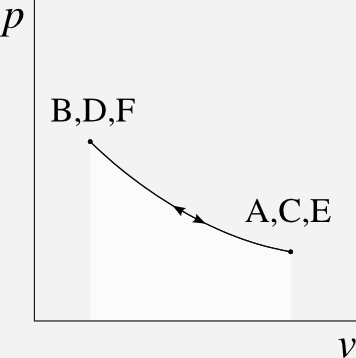
\includegraphics[width=3cm]{images/exe_pv_rev.png}
							\end{center}
						En revanche, pendant les évolutions rapides, à chaque trajet la pression finale est plus grande que ce qu’elle aurait été pendant un trajet lent :
							\begin{center}
								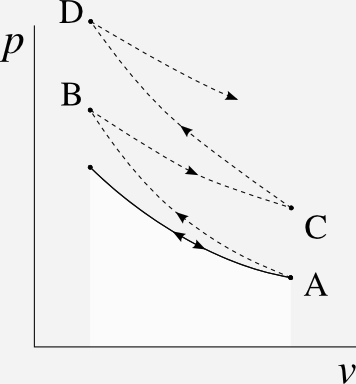
\includegraphics[width=3cm]{images/exe_pv_irr.png}
							\end{center}
						Ainsi, les propriétés s’élèvement progressivement sur le diagramme pression-volume : l’excédent de travail investi pendant les compressions, et le défaut de travail récupéré pendant la détente, se traduisent par une augmentation de l’énergie interne du gaz, dont la température augmente continuellement.
					\end{answer}
			\end{anexample}


	\subsection{La réversibilité}
	\label{ch_reversibilite}
	
		Prenons quelques instants pour réfléchir sur ce que nous venons de décrire. À chaque fois que nous comprimons un fluide «~trop vite~», il se passe quelque chose qui nous empêche de récupérer notre travail.
		
		Du point de vue de l’ingénieur/e, une évolution lente est un cas limite : celui où les dissipations sont minimisées. Par exemple, le travail qu’il faut investir pour comprimer un gaz jusqu’à~\SI{10}{\bar} est minimal lorsque la compression est réversible. De même, une turbine dans laquelle la détente est réversible extraira le maximum de travail d’un fluide comprimé. Et au contraire, dans un amortisseur automobile, on rend les évolutions très irréversibles pour qu’il fournisse lors du chemin retour un travail plus faible qu’à l’aller.
		
		\thermoquotebegin{O}
		D’où vient l’irréversibilité ? elle ne vient pas des lois de Newton. Si nous partons de l’idée que le comportement de toutes choses doit être en définitive compris en termes des lois de la physique et s’il apparaît également que toutes les équations ont cette propriété fantastique d’avoir une autre solution [valide] lorsque nous remplaçons $t$ par $-t$, alors chaque phénomène est réversible. Comment se fait-il alors que dans la nature, à une grande échelle, les choses ne soient pas réversibles ?
		\thermoquoteend{Richard Feynman, 1963}{\textit{The Feynman Lectures on \mbox{Physics}} \mbox{\cite{feynman1963, feynman1963fr}}\vspace{1em}} %handmade vspace
		Du point de vue de la physique, le phénomène d’irréversibilité est fascinant. En effet, nous partons de collisions de molécules, un phénomène tout à fait réversible, pour fabriquer une transformation irréversible : une évolution qui ne va que dans un sens ! Pour ramener le gaz dans l’état où il était avant de le comprimer brutalement, nous sommes obligés de lui prendre de la chaleur. Il est surprenant que sans aller à l’encontre des lois de Newton, nous ayons créé une situation où \emph{on ne peut pas revenir en arrière en «~faisant l’inverse~»}. Existe-t-il d’autres transformations irréversibles ? Peut-on quantifier l’irréversibilité ? Nous tenterons de répondre à ces questions dans les \courssept et \courshuit.

		En attendant, nous admettrons qu’il faut respecter trois conditions pour qu’une évolution soit réversible :

		\begin{enumerate}
			\item L’évolution doit se faire sans friction. Il ne doit pas y avoir de frottement dans les éléments mécaniques (par exemple, entre piston et cylindre).
			\item La pression dans le fluide doit être homogène. Le mouvement des parois doit donc être infiniment lent, et le fluide doit évoluer sans turbulence.
			\item La différence de température entre le fluide et son environnement doit être infiniment petite. Si de la chaleur est fournie ou rejetée, elle doit donc être transférée de façon infiniment lente.
		\end{enumerate}

		Ces trois conditions excluent évidemment toute évolution réelle --\ et en particulier, toute application pratique dans un moteur ! Toutefois, nous les utiliserons pour poser une limite théorique idéale à toutes les évolutions réelles que nous étudierons.



\section{Quantifier la chaleur avec un sy\-stème fer\-mé}

		Au risque de frustrer l’étudiant/e, il nous faut tout de suite avouer que \emph{nous ne savons pas quantifier directement les transferts de chaleur}. Nous allons toujours procéder par déduction : en quantifiant la variation d’énergie, et en y soustrayant les transferts sous forme de travail, on obtient la quantité de chaleur qui a été transférée. Mathématiquement, dans un système fermé, nous ne faisons que réutiliser l’\cref{eq_premier_principe_sf_maj} pour obtenir :
	\begin{IEEEeqnarray}{rCl}
		Q_{1 \to 2} 	& = & 	\Delta U \ - \  W_{1 \to 2} \\
		q_{1 \to 2} 	& = & 	\Delta u \ - \  w_{1 \to 2}
	\end{IEEEeqnarray}
	\begin{equationterms}
		\item pour un système fermé.
	\end{equationterms}
		
		Toute la difficulté pour quantifier un transfert de chaleur est maintenant de prédire et quantifier le changement de l’énergie interne, $\Delta U$. Pour les gaz, $U$ est quasiment proportionnelle à la température ; pour les liquides et vapeurs, la relation est plus complexe. Nous apprendrons à quantifier l’énergie dans les fluides aux \coursquatre et \courscinq.

\atstartofhistorysection
\section[Un peu d’histoire : le moteur compound]{Un peu d’histoire :\onlyamphibook{\\} le moteur compound}
\label{ch_histoire_compound}

	Dans les années 1830, le moteur à vapeur vient de révolutionner le paysage et le réseau économique de la Grande-Bretagne. Tout ou presque y voyage alors par rail : passagers, récoltes, charbon, produits de l’industrie. Ces trains sont tractés par des moteurs à vapeur, aux dimensions monumentales et à l’efficacité déplorable — quatre-vingt dix-sept pourcent de l’énergie dégagée par le charbon est perdue dans les cheminées. Ce n’est pas dramatique : le charbon et l’eau abondent, et il suffit d’arrêts ponctuels le long des lignes de chemin de fer pour réapprovisionner les machines.

	Sur les océans par contre, on utilise encore le vent pour se déplacer. Pour pouvoir joindre deux continents au moteur (c’est à dire sans louvoyer !), il faut résoudre deux problèmes.

	Le premier est que les moteurs consomment beaucoup d’eau. L’eau de mer, certes abondante, est inutilisable en l’état car les dépôts de sel et de calcaire provoqués lors de son ébullition étouffent les chaudières et entraînent un grave risque d’explosion. Il faut donc la désaliniser si l’on veut l’insérer dans la chaudière, ce qui est très coûteux en énergie.

	Le problème sera résolu avec l’utilisation des \textit{condenseurs}, dont les locomotives étaient dispensées par économie de place. Désormais, lorsque la vapeur a effectué son travail dans les cylindres, elle n’est plus simplement jetée dans l’atmosphère, mais refroidie dans de grands condenseurs avant d’être comprimée puis ré-insérée dans la chaudière. L’eau circule donc de façon cyclique à travers tout le moteur --\ il n’est plus besoin que de pallier les fuites.

	Le second problème est plus grave et plus difficile à résoudre : comment augmenter le rendement ? Ce n’est pas qu’une question financière : le premier navire transatlantique à vapeur, le \textit{SS Savannah}, est si inefficace qu’il termine sa traversée à la voile, alors qu’il n’était empli \emph{que} du charbon de son moteur !

	\begin{figure}
		\begin{center}
			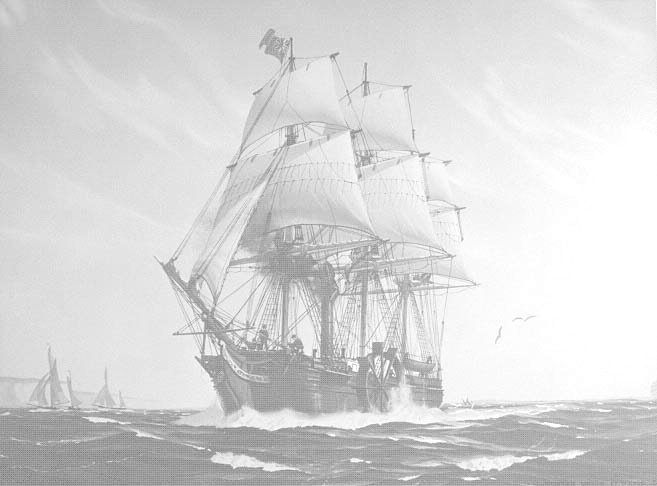
\includegraphics[width=0.7\textwidth]{images/ss_savannah.jpg}
		\end{center}
		\supercaption{\textit{SS Savannah}, première traversée atlantique à vapeur en 1819, terminée à la voile.}{Image \pd \wcfile{SS-Savannah.jpg}{par Hunter Wood, 1819}}
	\end{figure}

	Pour augmenter le rendement d’un moteur de capacité donnée, on cherche à augmenter la quantité de travail générée par chaque kilo de vapeur, qui peut être approximée par la relation~\ref{eq_travail_pdv} :

	\begin{equation*}
	w_\fromatob = - \int _{\A}^\B {p \diff v}
	\end{equation*}

	La première chose à faire est d’augmenter la pression $p_A$ de la vapeur, c’est à dire sa pression avant qu’elle ne débute sa détente dans les cylindres. Ce n’est pas chose facile : augmenter la pression de la chaudière augmente les contraintes structurelles qu’elle subit, donc son coût, et réduit son efficacité car les parois doivent être épaissies et alourdies.

	On peut ensuite tenter d’augmenter le $\Delta v $, c’est-à-dire la variation totale de volume lors du mouvement du piston. Autrement dit, il faut augmenter le volume balayé par les cylindres. Là encore, ce n’est pas chose facile.
	
	D’une part, lorsque l’on augmente le diamètre des cylindres --\ ce qui augmente l’aire~$S$\ -- on soumet les pistons à une plus grande force $F_A$, pour une pression $p_A$ donnée (\ref{def_pression}) :
	\begin{equation*}
	p \equiv \frac{F}{S}
	\end{equation*}
	En augmentant la force transmise, on atteint rapidement les limites structurelles de la mécanique motrice.

	D’autre part, lorsque l’on augmente la longueur des cylindres, on rallonge également le moteur et on alourdit considérablement le mécanisme de bielle et vile\-brequin. D’autant que la pression et le volume de la vapeur sont liés l’un à l’autre : ils suivent approximativement une relation de type $p v^{x} = k$ pendant la détente. Autrement dit, plus le volume augmente, plus la pression diminue : au fur et à mesure que l’on rallonge le cylindre, les gains en travail sont de plus en plus faibles.

	Le moteur \vocab[compound!moteur, principe]{compound} répond à ce problème en utilisant plusieurs cylindres \textit{en série} (\cref{fig_cylindres_compound}). La vapeur à haute pression déplace d’abord un piston de petit diamètre (limitant ainsi la force exercée sur le mécanisme). Ensuite, elle est transférée dans un autre cylindre, de plus grand diamètre. Celui-ci permet d’obtenir une force identique avec une pression plus basse ; il balaie un plus grand volume.

	\begin{figure}
		\begin{center}
			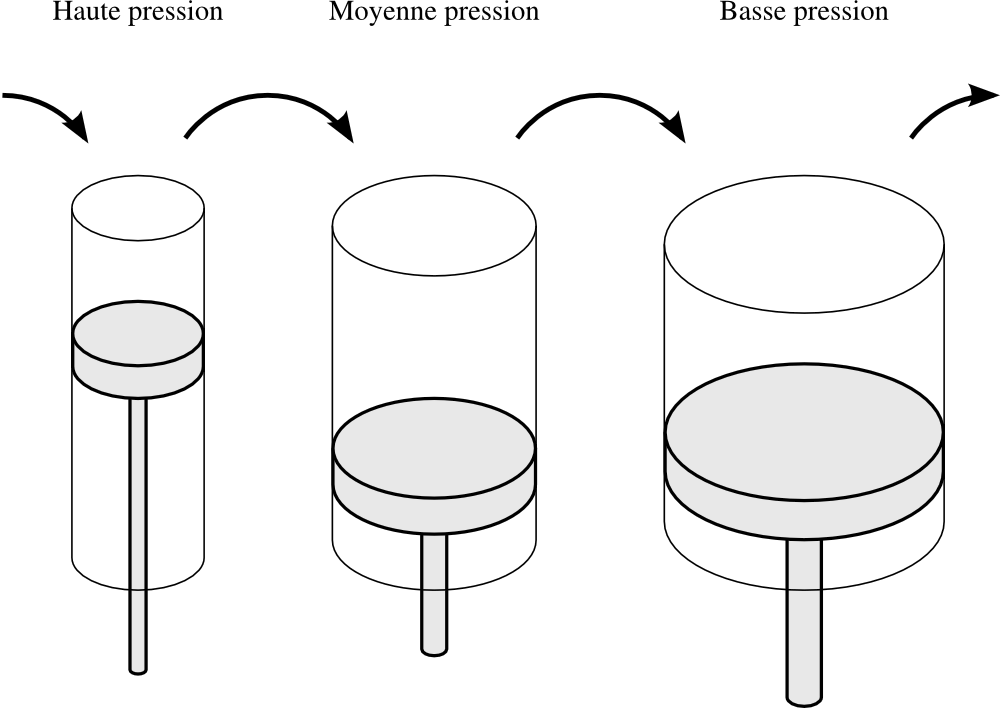
\includegraphics[width=0.8\textwidth]{images/cylindres_compound.png}
			\onlyamphibook{\vspace{-1cm}}%handmade pour tout faire tenir sur 1 page
		\end{center}
		\onlyamphibook{\supercaption{Cylindres en série, dits \textit{compound}.}{schéma \ccbysa \olivier}}
		\onlyframabook{\supercaption{Cylindres en série, dits \textit{compound}.\\\scriptsize\slshape Schéma \ccbysa \olivier\normalsize\upshape}{}}
		\label{fig_cylindres_compound}
			\onlyamphibook{\vspace{-1em}}%handmade, grave
	\end{figure}

	Ainsi, en augmentant le volume total balayé par la vapeur en expansion, on peut extraire plus de travail de la vapeur compressée, sans surdimensionner le vilebrequin ni surcharger les pistons.

	Avec un tel moteur, la marine marchande est capable d’abandonner le cabotage : elle s’empare de cette nouvelle technologie qui connaît un succès immédiat. De deux cylindres en série (\vocab[compound!double]{double compound}) on passe à trois, et même parfois quatre (\vocab[compound!quadruple]{quadruple compound} !), pour extraire de la vapeur à chaque fois plus d’énergie, sous forme de travail.

	\begin{figure}
		\begin{center}
			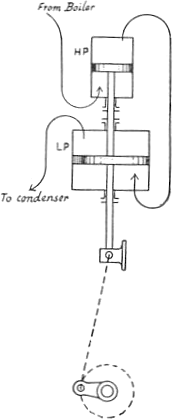
\includegraphics[height=11cm, max height=0.55\textheight]{images/ripper_compound_1.png}
			\onlyframabook{\hspace{0.5cm}}
			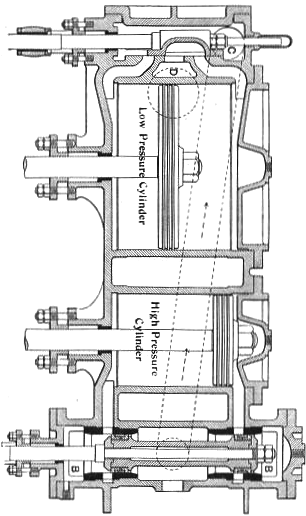
\includegraphics[height=11cm, max height=0.55\textheight]{images/ripper_compound_2.png}
		\end{center}
		\onlyamphibook{\supercaption{Différents systèmes compound à vapeur.}{\wcfile{Compound engine with both piston and slide valves (Heat Engines, 1913).png}{Images par Prof. William Ripper, 1889}}}
		\onlyframabook{\supercaption{Différents systèmes compound à vapeur.\\\scriptsize\slshape \wcfile{Compound engine with both piston and slide valves (Heat Engines, 1913).png}{Images par Prof. William Ripper, 1889} (\pd)}{}}
		
	\end{figure}

	L’enthousiasme gagne les armateurs, qui se targuent désormais ne plus devoir brûler qu’une feuille de papier pour déplacer une tonne de cargaison sur un mile. Même s’il s’entend que ledit papier est fort épais, l’avancée est faite. Voilà le thé des Indes bientôt dans les tasses londoniennes --\ l’empire britannique dispose à partir de ce moment des machines dont avait besoin son formidable réseau économique.
\atendofhistorysection


\atstartofexercices
	\subsubsection{Évolutions simples}
\label{exo_evolutions_simples}

	(un exercice simplement destiné à mettre en pratique les conventions de signe et le vocabulaire du cours)

	Une masse de~\SI{400}{\gram} d’eau est placée dans un réservoir hermétique. Elle suit une évolution pendant laquelle elle reçoit \SI{50}{\kilo\joule\per\kilogram} de chaleur et voit son énergie interne augmenter de~\SI{4}{\kilo\joule}.
	
	\begin{enumerate}
		\item A-t-elle reçu ou fourni du travail, et en quelle quantité ?
	\end{enumerate}
	
	On fournit ensuite à cette même masse un travail de~\SI{800}{\joule} de manière adiabatique.
	
	\begin{enumerate}
		\shift{1}
		\item Quelle est la variation de son énergie interne spécifique ?
	\end{enumerate}
	

\subsubsection{Évolutions arbitraires d’un gaz en laboratoire}
\label{exo_evolutions_arbitraires}

	Une masse de~\SI{80}{\gram} d’hélium est contenue dans un cylindre de~\SI{0,04}{\metre\cubed}. Le gaz est d’abord refroidi de façon réversible à pression constante jusqu’à~\SI{0,02}{\metre\cubed} et~\SI{2}{\bar} ; puis réchauffé à volume constant jusqu’à~\SI{4}{\bar}.
	
	\begin{enumerate}
		\item Tracez l’évolution sur un diagramme pression-volume.
		\item Quel est le travail fourni ou reçu par le gaz ?
	\end{enumerate}


\subsubsection{Suspension pneumatique de camion}
\label{exo_pneumatique_camion}

	Le système de suspension pneumatique d’une remorque de camion contient avec un réservoir d’air. Lorsque la remorque est chargée, les pistons qui la relient au chassis descendent, l’air qui du réservoir (\cref{fig_camion}).

	\begin{figure}
	\begin{center}
		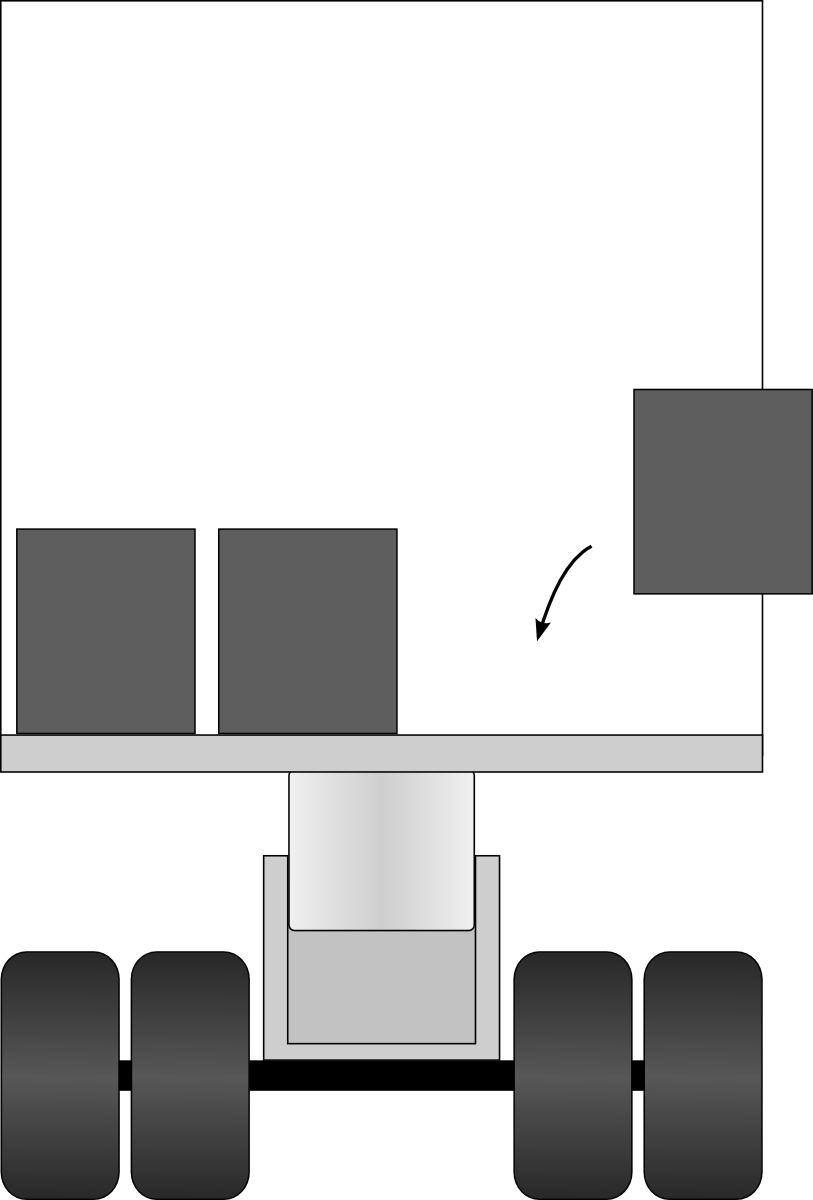
\includegraphics[height=8cm]{images/piston_camion.png}
	\end{center}
		\supercaption{Modélisation schématique d’un système de suspension pneumatique de camion. Le piston, au centre, comprime une masse d’air (en bleu) lorsque la remorque est chargée.}{schéma \cczero \oc}
	\label{fig_camion}
	\end{figure}
	
	Dans un premier temps on charge le camion très progressivement. L’air à l’intérieur du cylindre ne perd ni reçoit de chaleur. Ses caractéristiques évoluent alors selon la relation $p v^{1,4} = \num{5,438e4}$ (en unités \textsc{si}).
	
	La compression commence à $p_\A = \SI{2,5}{\bar}$. Lorsque le chargement est terminé, la pression est montée à $p_\B = \SI{10}{\bar}$. 
	
	\begin{enumerate}
		\item Tracez qualitativement l’évolution du gaz pendant le chargement sur un diagramme pression-volume.
		\item Le travail effectué par une force $\vec F$ sur un déplacement $\vec l$ s’exprime selon
			\begin{equation}
				W \equiv \vec F \cdot \vec l 	\tag{\ref{eq_travail_fdl}}
			\end{equation}
			À partir de cette équation, exprimez le travail effectué sur un corps de masse fixe en fonction de son volume spécifique et de sa pression interne.
		\item Combien d’énergie le gaz a-t-il reçu pendant le chargement ?
		\item Quelle énergie le gaz fournirait-il en retour si le camion était déchargé très progressivement ?
	\end{enumerate}
	
	On décharge brutalement le camion et le piston remonte rapidement jusqu’à ce que la pression finale redescende à sa valeur initiale.
	
	\begin{enumerate}
		\setcounter{enumi}{3}
		\item Tracez qualitativement l’évolution sur le diagramme pression-volume précédent.
		\item Que peut-on faire pour ramener le gaz à l’état exact où il était avant le chargement ?
	\end{enumerate}


\subsubsection{Compresseur à air}
\label{exo_compresseur_air}

	Dans un petit compresseur à air (\cref{fig_compresseur}), un piston comprime lentement et sans frottement une masse fixe d’air. Le cylindre est muni d’aubes, qui permettent de dissiper de la chaleur. Ainsi, la compression se fait à énergie interne constante.	

	\begin{figure}
	\begin{center}
		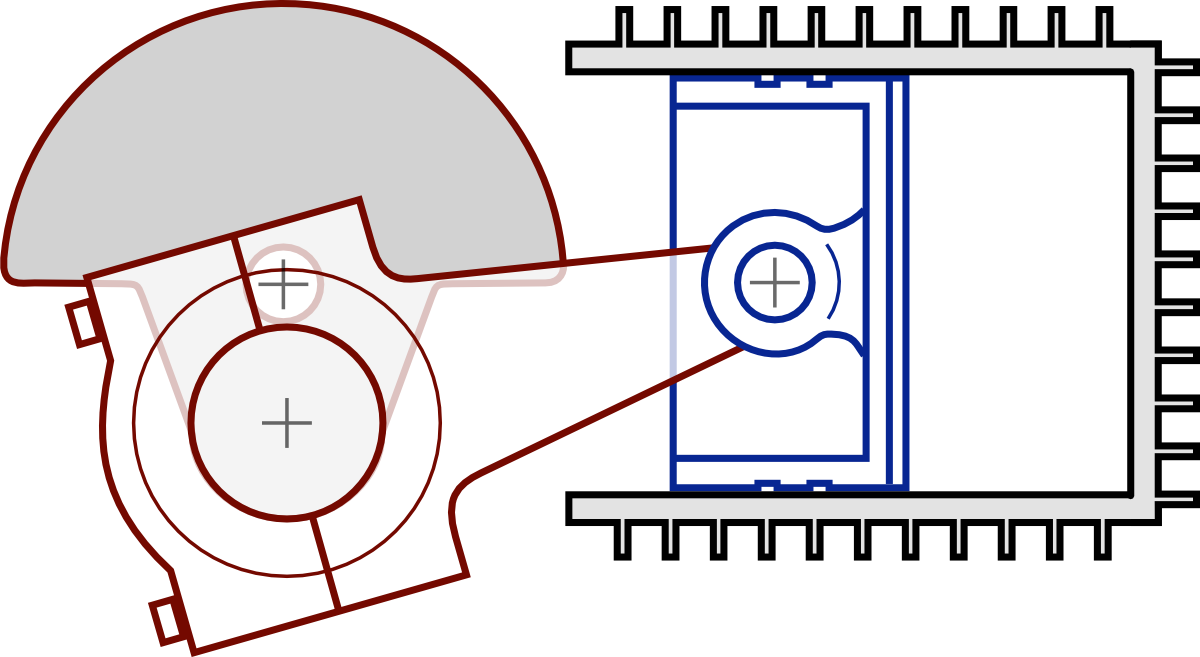
\includegraphics[width=8cm]{images/compresseur_air.png}
	\end{center}
	\supercaption{Schéma de coupe d’un petit compresseur à air à piston. Les soupapes d’admission et de sortie ne sont pas représentées.}{Schéma \ccbysa \wcfile{Piston_bielle_vilebrequin_coupe_et_schema_cinematique.svg}{Christophe Dang Ngoc Chan} \& \olivier}
	\label{fig_compresseur}
	\end{figure}

	On dépense, pour la compression de l’air, un travail de~\SI{150}{\kilo\joule\per\kilogram}. 
		
	\begin{enumerate}
		\item Quel est le transfert de chaleur pendant la compression ?
	\end{enumerate}
	
	Avant de commencer la compression, l’air est à pression et masse volumique atmosphériques (\SI{1}{\bar} ; \SI{1,2}{\kilogram\per\metre\cubed}). Le diamètre du cylindre est de~\SI{5}{\centi\metre} et sa profondeur intérieure est de~\SI{15}{\centi\metre}.
	
	\begin{enumerate}
		\shift{1}
		\item Quelle est la masse d’air incluse dans le cylindre ?
	\end{enumerate}


	Pendant la compression, on observe que la pression et le volume spécifique sont liés par la relation $p v = k$ (où $k$ est une constante). 

	\begin{enumerate}
		\shift{2}
		\item À quelle pression va-t-on pouvoir mener l’air à la fin de la compression ?
	\end{enumerate}


\subsubsection{Cycle d’un moteur à essence}
\label{exo_cycle_moteur_essence}

	On souhaite étudier le fonctionnement d’un moteur à essence à quatre cylindres (\cref{fig_exo_pistons}). Comme tous les moteurs thermiques alternatifs, il dégage du travail en faisant varier la pression et le volume de petites quantités d’air emprisonnées dans ses cylindres. Nous simplifions ici les détails de son fonctionnement pour le réduire au cas idéal, dans lequel les évolutions sont toutes réversibles.
	
	Le moteur a pour cylindrée \SI{1,1}{\liter} ; il est muni de quatre cylindres de diamètre \SI{7}{\centi\metre} et a un taux de compression (rapport entre volumes maximum et minimum dans un cylindre) de~\num{7,9}. L’air pénètre dans le moteur aux conditions atmosphériques (\SI{1}{\bar}, \SI{0,84}{\metre\cubed\per\kilogram}).
	
		\begin{figure}
			\begin{center}
				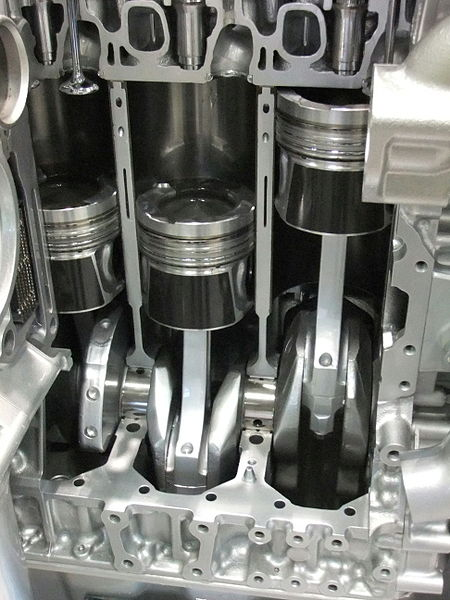
\includegraphics[width=6cm, max width=0.8\columnwidth]{images/pistons_cutaway.jpg}
			\end{center}
			\supercaption{Pistons et cylindres d’un moteur automobile découpé.}{\wcfile{Internal combustion engine pistons of partial cross-sectional view.jpg}{Photo} \ccbysa par \wcu{Mj-bird}}
			\label{fig_exo_pistons}
		\end{figure}
	
	Nous pouvons décrire un cycle à l’intérieur d’un cylindre avec les quatre étapes suivantes :
	
	\begin{description}
			\item [De A à B] l’air est comprimé de façon adiabatique réversible depuis le point mort bas jusqu’au point mort haut. Pendant cette évolution, nous savons que ses propriétés sont liées par la relation $p \ v^{k_1} = k_2$. En B, la pression a atteint \SI{16,97}{\bar}. 
			\item [De B à C] il est chauffé à volume constant (comme si le piston était immobilisé), jusqu’à ce que la pression atteigne~\SI{75}{\bar}. En mesurant la température on constate que son énergie interne spécifique augmente de~\SI{1453,3}{\kilo\joule\per\kilogram}.
			\item [De C à D] l’air est détendu de façon adiabatique réversible depuis le point mort haut jusqu’au point mort bas. Ses propriétés sont liés par la relation $p \ v^{k_1} = k_3$.
			\item [De D à A] il est refroidi à volume constant (comme si le piston était immobilisé), jusqu’à retrouver ses propriétés en A.\\
				(En pratique, cette phase de refroidissement a lieu hors du moteur, dans l’atmosphère. Elle peut toutefois être modélisée ainsi sans induire d’erreur.)
	\end{description}

	\begin{enumerate}
		\item Tracez qualitativement le cycle suivi par l’air sur un diagramme pression-volume.
		\item {Quelle est la masse d’air présente dans un cylindre ?\\
				{\tiny indice : $V_\text{cylindrée} = 4 (V_\text{cylindre max.} - V_\text{cylindre min.}) = 4 (V_\text{point mort bas} - V_\text{point mort haut})$}}
		\item Quel est le travail spécifique reçu par l’air pendant la compression (de A à B) ?
		\item Quelle est la chaleur spécifique reçue par l’air pendant la combustion (de B à C) ?
		\item Quel est le travail spécifique dégagé par l’air pendant la détente (de C à D) ?
		\item Quelle est la chaleur spécifique rejetée par l’air pendant la phase de refroidissement ?
		\item Quelle est l’efficacité du moteur, c’est à dire le rapport entre le travail net dégagé pendant le cycle et la chaleur fournie pendant la combustion ?
		\item Combien faut-il effectuer de cycles par seconde pour que le moteur dégage une puissance de~\SI{80}{\cheval} (\SI{58,84}{\kilo\watt}) ?
	\end{enumerate}



\subsubsection{Travail dans un moteur diesel}
\label{exo_quatre_cylindres}
	
	Nous étudions le fonctionnement d’un moteur alternatif à quatre cylindres en modélisant son fonctionnement dans le cas le plus favorable, c’est à dire avec des évolutions très lentes (parfaitement réversibles).

	\begin{figure}
		\begin{center}
			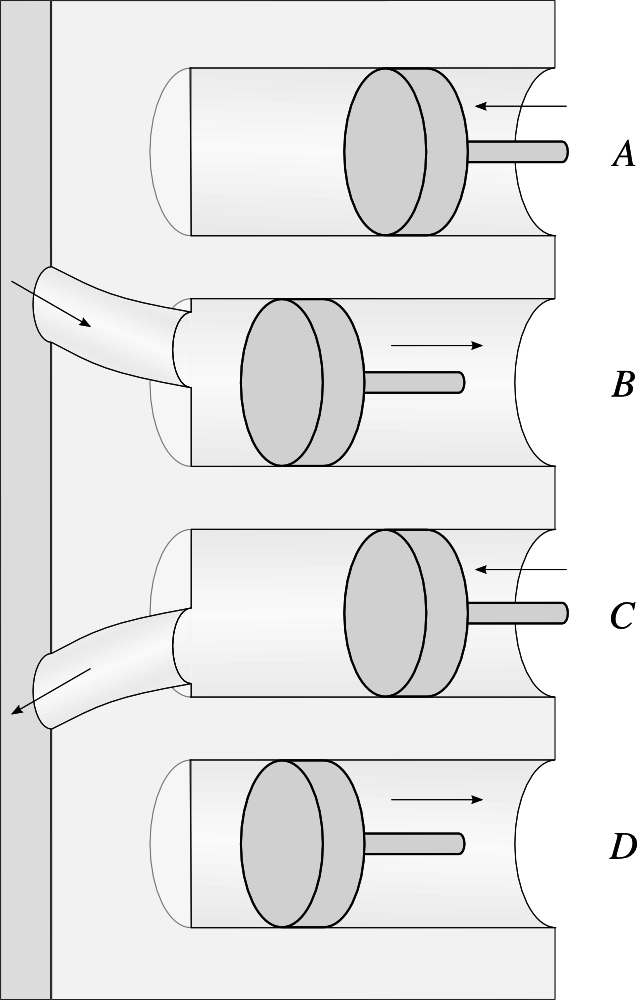
\includegraphics[width=8cm]{images/quatre_cylindres.png}
		\end{center}
		\supercaption{Représentation schématique du fonctionnement d’un moteur à quatre cylindres. Les pistons A et C sont en remontée, et les pistons B et D sont en descente. Ils sont tous les quatre liés au même axe moteur, non représenté ici.}{Schéma \ccbysa \olivier}
		\label{fig_quatre_cylindres}
	\end{figure}
	
	À l’intérieur du bloc moteur schématisé en \cref{fig_quatre_cylindres}, quatre pistons liés à l’axe moteur par un vilebrequin (non représenté) sont en mouvement. L’évolution est différente dans chaque cylindre :
	
	\begin{description}
		\item [Cylindre A :] {compression (l’air restant prisonnier du cylindre).\nopagebreak\\
									La compression de l’air débute à \SI{0,8}{\bar} et ses y sont liées par la relation $p V^{\num{1,3}} = k_1$.}
		\item [Cylindre B :] {admission.\\
									L’air est admis à pression constante de~\SI{0,8}{\bar}.}
		\item [Cylindre C :] {échappement.\\
									L’air est rejeté à pression constante de~\SI{1,1}{\bar}.}
		\item [Cylindre D :] {détente.\\ 
									L’air à haute pression et température est prisonnier du cylindre ; ses propriétés sont aussi reliées par la relation $p V^{\num{1,3}} = k_2$.}
	\end{description}
		
		Bien sûr, le rôle de chaque cylindre change deux fois par tour. Nous étudions ici les transferts de travail sur un demi-tour moteur.

		Même si les cylindres B et C ne sont pas des systèmes fermés, nous pouvons ici modéliser leurs évolutions comme si c’était le cas, sans induire d’erreur.

		Les conditions atmosphériques sont de~\SI{1}{\bar} et \SI{1,225}{\kilogram\per\metre\cubed}.	La cylindrée du moteur est de~\SI{1,5}{\liter} et le taux de compression (c’est à dire le rapport des volumes minimal et maximal au sein de chaque cylindre) est de~\num{22}. 
		
		\begin{enumerate}
			\item Représentez qualitativement l’évolution dans chacun des cylindres sur un même diagramme pression-volume.
			\item Quelle est l’énergie nécessaire pour déplacer les cylindres B et C ?
			\item Quelle est l’énergie reçue par le gaz dans le cylindre A ?
		\end{enumerate}
		
		On souhaite que le moteur développe une puissance de~\SI{30}{\kilo\watt} à vitesse de~\num{2000} \si{tours/min}. Ses pertes mécaniques sont de l’ordre de~\SI{15}{\percent}.
		
		\begin{enumerate}
			\shift{3}
			\item Quel est le travail qui doit être développé par le cylindre D pendant la détente ?
			\item À quelle pression la combustion de l’essence dans le cylindre D doit-elle y porter l’air, pour que la détente puisse faire fonctionner le moteur ?
		\end{enumerate}



\subsubsection{Prendre de la chaleur où il fait plus froid}
\label{exo_prendre_de_la_chaleur}

	Un/e étudiant/e tente une expérience avec un peu d’air dans un cylindre, dont il/elle contrôle le volume avec un piston. Le but est de prélever de la chaleur à l’extérieur, où la température est basse, pour la rejeter à l’intérieur de la pièce.

	La masse d’air emprisonnée dans le cylindre est de~\SI{6e-3}{\kilogram}.
	
	Au départ, l’air dans le cylindre occupe un volume de~\SI{0,5}{\liter}. La pression et la température sont celles de la pièce (\SI{1}{bar} ; \SI{18}{\degreeCelsius}).

	\begin{description}
		\item[de A à B] L’étudiant/e isole bien le cylindre avec un isolant thermique, et détend lentement le gaz en augmentant son volume jusqu’à~\SI{4,5}{\liter}. Nous savons\footnote{Nous verrons d’où vient cette relation et apprendrons à calculer cette température au \coursquatre.} que pendant ce type de détente, la pression et le volume sont liés par la relation 
			\begin{equation*}
				p v^{1,4} = k_2
			\end{equation*}
			 où $k_2$ est une constante. 
		
			La température du gaz chute dramatiquement pendant la détente\ – en B le thermomètre indique finalement $T_\B = \SI{121}{\kelvin}$. 
		
		\item[de B à C]	L’étudiant/e fixe le volume du cylindre en bloquant mécaniquement le piston, retire l’isolant thermique, et pose le cylindre au dehors du bâtiment (température extérieure : \SI{-5}{\degreeCelsius}). La température et la pression du gaz remontent doucement.

		\item[de C à A] Lorsque la pression atteint \SI{1}{\bar} précisément, la température de l’air est indiquée à~$T_\C = \SI{262}{\kelvin}$. 	
					
			L’étudiant/e souhaite revenir aux conditions de départ (en réduisant le volume jusqu’au volume initial) en gardant la pression constante à~\SI{1}{\bar}.
	\end{description}.
	
	\begin{enumerate}
		\item Schématisez l’évolution sur un diagramme pression-volume.
		\item {Montrez que lors d’une évolution réversible d’un sytème fermé dont les propriétés sont liés par une relation de type $p v^{k_1} = k_2$ (où $k_1 \neq 1$ et $k_2$ sont des constantes), le travail spécifique développé est :
				\begin{equation*}
				w_{\A\to\B} = \frac{p_\B v_\B - p_\A v_\A}{k_1 - 1}
				\end{equation*}}
		\item Quel est le travail spécifique fourni par le gaz pendant la détente ?
		\item La capacité thermique de l’air lorsque l’on bloque son volume est égale à~\SI{718}{\joule\per\kilo\gram\per\kelvin}. Quelle quantité de chaleur a-t-elle été rejetée ou prélevée de l’air extérieur ?
		\item Quelle quantité de travail sera nécessaire pour effectuer le retour C$\to$ A à pression constante ?
		\item Sur l’entièreté du cycle, l’étudiant/e aura-t-il ou elle dépensé ou reçu du travail ?
		\item {[question difficile]} Le chemin du retour à pression constante nécessite un transfert de chaleur. Dans quel sens, et en quelle quantité ? Pourquoi ce transfert ne peut-t-il (malheureusement) pas être entièrement effectué à l’intérieur du bâtiment ?
	\end{enumerate}



\exercisesolutionpage
\subsubsection*{Résultats}
	\linktosolutionsblurb

	\begin{description}
		\item [\ref{exo_evolutions_simples}]
						\tab 1) $W_\fromatob = \Delta U - m q_\fromatob = \SI{-16}{\kilo\joule}$ (donc un travail fourni)
						\tab 2) $\Delta u = q_\frombtoc + w_\frombtoc =  0 + \frac{W_\frombtoc}{m} = \SI{+2}{\kilo\joule\per\kilogram}$.
		\item [\ref{exo_evolutions_arbitraires}]
						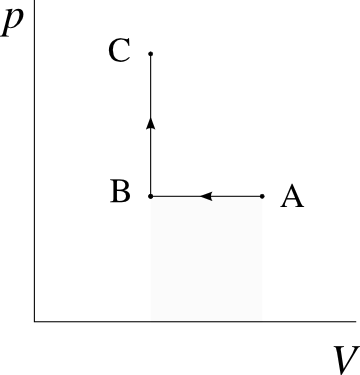
\includegraphics[width=2.5cm]{images/exo_pv_1.png}
						\tab 2) $W_{\A\to\C} = W_\fromatob + W_\frombtoc = -p_{\text{cste.}} \left[V\right]_{V_\A}^{V_\B } + 0 = \SI{+4}{\kilo\joule}$
		\item [\ref{exo_pneumatique_camion}]
						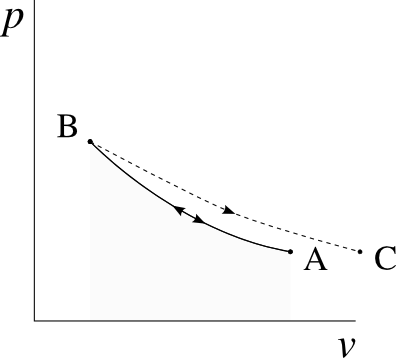
\includegraphics[width=2.5cm]{images/exo_pv_camion.png}
						\tab 2) voir \S\ref{ch_travail_pdv} \& \S\ref{ch_travail_fdl}
						\tab 3) $v_\A = \SI{0,336}{\metre\cubed\per\kilogram}$ et $v_\B = \SI{0,125}{\metre\cubed\per\kilogram}$ ; ainsi $w_\fromatob = -k \left[\frac{1}{\num{-0,4}} v^{\num{-0,4}}\right]_{v_\A}^{v_\B } = \SI{+102,1}{\kilo\joule\per\kilogram}$.
						\tab 4) $w_\frombtoa =  - w_\fromatob$
						\tab 5) Un refroidissement à pression constante, par exemple.
		\item [\ref{exo_compresseur_air}] 
						\tab 1) $q_\fromatob = \Delta u - w_\fromatob = - w_\fromatob$. 
						\tab 2) $m = \frac{V_\A}{v_\A} = \SI{3,534e-4}{\kilogram}$
						\tab 3) $\frac{v_\B }{v_\A} = \exp \left[-\frac{w_\fromatob}{k}\right]$ ; ainsi  $p_\B = p_\A \frac{v_\A}{v_\B } = \SI{6,05}{\bar}$
		\item [\ref{exo_cycle_moteur_essence}]
						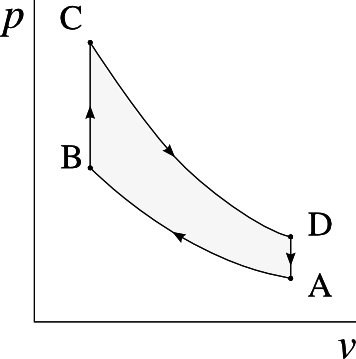
\includegraphics[width=2.5cm]{images/exo_pv_moteur_essence.png}
						\tab 2) $V_\A = \SI{3,149e-4}{\metre\cubed}$ ; ainsi $m_\A = \frac{V_\A}{v_\A} = \SI{3,748e-4}{\kilogram}$
						\tab 3) $k_1 = \num{1,3699}$ et $k_2 = \SI{7,8753e4}{\usi}$ ; ainsi $w_\fromatob = -k_2 \left[\frac{1}{-k_1 + 1} v^{-k_1 + 1} \right]_{v_\A}^{v_\B } = \SI{+260,7}{\kilo\joule\per\kilogram}$.
						\tab 4) $q_\frombtoc = \Delta u - w_\frombtoc = \Delta u - 0 = \SI{+1543,3}{\kilo\joule\per\kilogram}$
						\tab 5) $w_\fromctod = -k_3 \left[\frac{1}{-k_1 + 1} v^{-k_1 + 1} \right]_{v_\C}^{v_\D} = -\frac{k_3}{k_2} w_\fromatob = -\frac{p_\C}{p_\B } w_\fromatob = \SI{-1152,2}{\kilo\joule\per\kilogram}$
						\tab 6) $q_\fromdtoa = -w_\fromatob - q_\frombtoc - w_\fromctod = \SI{-651,8}{\kilo\joule\per\kilogram}$
						\tab 7) $\eta_{\text{moteur}} = \left|\frac{w_\fromatob + w_\fromctod}{q_\frombtoc}\right| = \SI{57,8}{\percent}$ (très honorable)
						\tab 8) $f = \frac{\dot W_{\text{moteur}}}{m_\A \ (w_\fromatob + w_\fromctod)} = \SI{176,1}{\hertz}$ (176 combustions par seconde), soit environ \SI{5300}{tours par minute} avec un moteur quatre cylindres à quatre temps.
		\item [\ref{exo_quatre_cylindres}]
						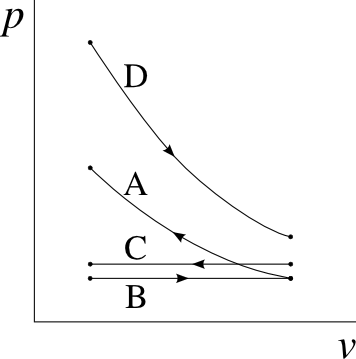
\includegraphics[width=2.5cm]{images/exo_pv_quatre_cylindres.png}
						\tab 2) $W_{\text{cyl. B}} = -p_\B \left[V\right]_{V_\text{min.}}^{V_\text{max.}} = - p_\B \left(\frac{V_\text{cylindrée}}{4}\right) = \SI{-30}{\joule}$ ; $W_{\text{cyl. B}} =  \SI{-41,3}{\joule}$
						\tab 3) $V_\text{A1} = \frac{22}{21\times4}V_\text{cylindrée} = \SI{3,9286e-4}{\metre\cubed}$ et $V_\text{A2} = \frac{V_\text{A1}}{22} = \SI{1,7857e-5}{\metre\cubed}$. Ainsi, $k_1 = \SI{2,9895}{\usi}$, et enfin $W_{\text{cyl. A}} = \frac{k_1}{\num{0,3}} \left(V_\text{A2}^{\num{-0,3}} - V_\text{A1}^{\num{-0,3}}\right) = \SI{+185,5}{\joule}$.
						\tab 4) $\dot n = \SI{2000}{rpm} = \SI{33,3}{rps}$ : il y a donc \num{66,7} évolutions par seconde ($f = \SI{66,7}{\hertz}$). On obtient $W_\text{4 cylindres} = \frac{1}{f} \frac{1}{\eta_\text{méca.}} \dot W_\text{moteur}$ ; et enfin $W_\text{cyl. D} = W_\text{4 cylindres} - W_\text{cyl. A} - W_\text{cyl. B} -W_\text{cyl. C} = \SI{-726,2}{\joule}$. 
						\tab 5) On calcule $k_2$ à partir de $W_\text{cyl. D}$, et on obtient $p_\text{D1} = \SI{173,9}{\bar}$.
		\item [\ref{exo_prendre_de_la_chaleur}] 
						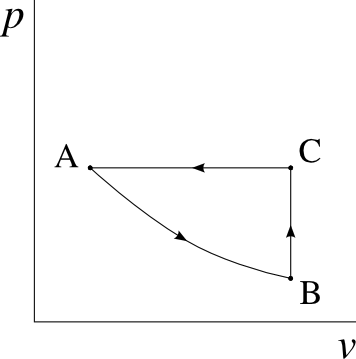
\includegraphics[width=2.5cm]{images/exo_pv_prelever.png}
						\tab 3) Ayant obtenu $p_\B = \SI{4,61e-2}{\bar}$, on calcule $W_\fromatob = \frac{p_\B V_\B - p_\A V_\A}{k_1 - 1} = \SI{-73,14}{\joule}$.
						\tab 4) $Q_\frombtoc = m c_v \Delta T = \SI{+607,4}{\joule}$
						\tab 5) $W_{\C \to \A} = \SI{+400}{\joule}$ (facile!)
						\tab 5) $W_\text{cycle} = \SI{+326,86}{\joule}$, donc une dépense de l’étudiant/e.
						\tab 6) $Q_{\C \to \A} = \SI{-934,26}{\joule}$
						\tab 7) C’est une histoire de température\ldots
	\end{description}


\atendofexercices
